\chapter{Evaluation}\label{chap:evaluation}

This section reflects the results of all the testing performed with the different programming languages and architectures / types of computer.

\begin{table}[ht]
  \centering
  \begin{tabular}{lccccc}
    \toprule
               & \gls{OS}       & C++                  & Go       & Python & PyPy \\
    \midrule
    Server     & Ubuntu 24.04.2 &  GCC 14.2.0          & 1.24.2  & 3.12.3 & 7.3.19 \\
    Laptop     & macOS 15.5     &  Apple Clang 17.0.0  & 1.24.2  & 3.13.5 & 7.3.19 \\
    Raspberry  & Debian 12      &  GCC 14.2.0          & 1.24.4  & 3.13.5 & 7.3.19 \\
    Desktop    & Ubuntu 24.04.2 &  GCC 13.3.0          & 1.24.5  & 3.13.5 & 7.3.19 \\
    \bottomrule
  \end{tabular}
  \caption[Language versions and compilers per platform]{Programming languages versions and operating systems used.}
  \label{tab:lang-platforms}
\end{table}

\section{Measurement Platforms}

The benchmark is run 5 times to obtain a good average. \autoref{chap:appendix-number-benchmarks} shows the percentage change between different runs for different numbers of iterations.

\subsection{Many-Core Platform}

This platform represents the most powerful as well as power-hungry combination of all devices in my test suite. This is a rack server with two Intel Xeon Gold 6326 processors, each having 16 cores and 32 threads, contributing to a total of 32 cores and 64 threads. It also has the largest amount of \gls{ram} from this testing, with 256GB of \gls{DDR4} memory.

As it has two sockets (one per CPU chip), there must be intercommunication between these processors if a process spreads out to more than 32 threads, or is set by the user using the command \texttt{taskset}, which fixes the cores the process can run on.


\subsubsection{Cache \& Numa}
Regarding the cache of these processors, as it can be seen from \autoref{lst:xeon-cache}, the cache at level 1 has 32 instances of 1.5 MiB of data cache and 1 MiB of instruction cache, half the total number of virtual cores, which is 64. There is also 48MB of L3 cache for each of the two processors.

\begin{lstlisting}[language=bash, caption={Cache of the Intel Xeon Gold 6326}, label={lst:xeon-cache}]
$ lscpu | grep -i cache
Caches (sum of all):
  L1d:                    1.5 MiB (32 instances)
  L1i:                    1 MiB (32 instances)
  L2:                     40 MiB (32 instances)
  L3:                     48 MiB (2 instances)
NUMA:
  NUMA node(s):           2
  NUMA node0 CPU(s):      0-15,32-47
  NUMA node1 CPU(s):      16-31,48-63
\end{lstlisting}

\subsubsection{Core Configurations}

This system was the most versatile in terms of the number of tests that could be performed, as it has many processors and uses Linux on x86, providing a great advantage for forcing processes to run on specific cores.

The tests were conducted on a variety of core configurations, always setting cores in the same processor for core numbers less than 16.

\begin{itemize}
    \item \textbf{1 Core}: Testing with one core, producing the baseline for the program's energy consumption and execution time.
    \item \textbf{2 Cores}: Testing with 2 cores provides the first glimpse of parallelization benefits.
    \item \textbf{4 Cores}: Testing with 4 cores because many computers from some time ago had four cores.
    \item \textbf{8 Cores}: Testing with 8 cores gives us great insight into how many processors in the market work, and it is half the amount of cores inside one chip.
    \item \textbf{14 Cores}: Testing with 14 cores, because it is the number of cores available on the laptop and we wanted to have an execution time comparison.
    \item \textbf{16 Cores}: Testing with 16 cores as it is the amount of real cores on a single chip. This should be one of the most energy-efficient and fastest tests, if there were only one \gls{cpu}.
    \item \textbf{28 Cores (different \glspl{cpu}, all real cores, no logical cores)}: Testing with 28 cores distributed across two sockets is interesting because there has to be information sharing over the bus inside the motherboard to synchronize both \glspl{cpu}. This won't be as energy efficient, but may be faster.
    \item \textbf{28 Cores (same CPU, 16 cores, 32 virtual cores)}: Testing with 28 cores inside the same CPU; the performance should be slower as there are fewer real cores to tackle the work, but it has the advantage of not needing to share data with another socket.
    \item \textbf{32 Cores (same socket)}: Testing with 32 cores in the same socket uses all available logical threads of a system: the 16 real cores and the other 16 threads the \gls{cpu} has thanks to Hyper-Threading.
    \item \textbf{32 Cores (only real cores)}: Testing with 32 real cores across two sockets should be the most powerful combination for CPU-intensive tasks, as all operations should be able to be carried out without many interruptions.
    \item \textbf{48 Cores}: Testing with 48 cores forces us to use all real cores and some logical cores.
    \item \textbf{60 Cores}: Testing with 60 cores is also interesting (not 64), as this would force the machine to interrupt the program we are benchmarking to perform routine operations, such as checking for incoming connections or logging.
\end{itemize}

\subsubsection{Results}

\newlength{\plotwidthgraph}
\newlength{\plotheightgraph}
\setlength{\plotwidthgraph}{14cm}
\setlength{\plotheightgraph}{8cm}

The results for the server are shown in the following figures and tables. The energy consumption is measured in joules, and the execution time is measured in seconds. 

\begin{figure}[H]
  \centering
  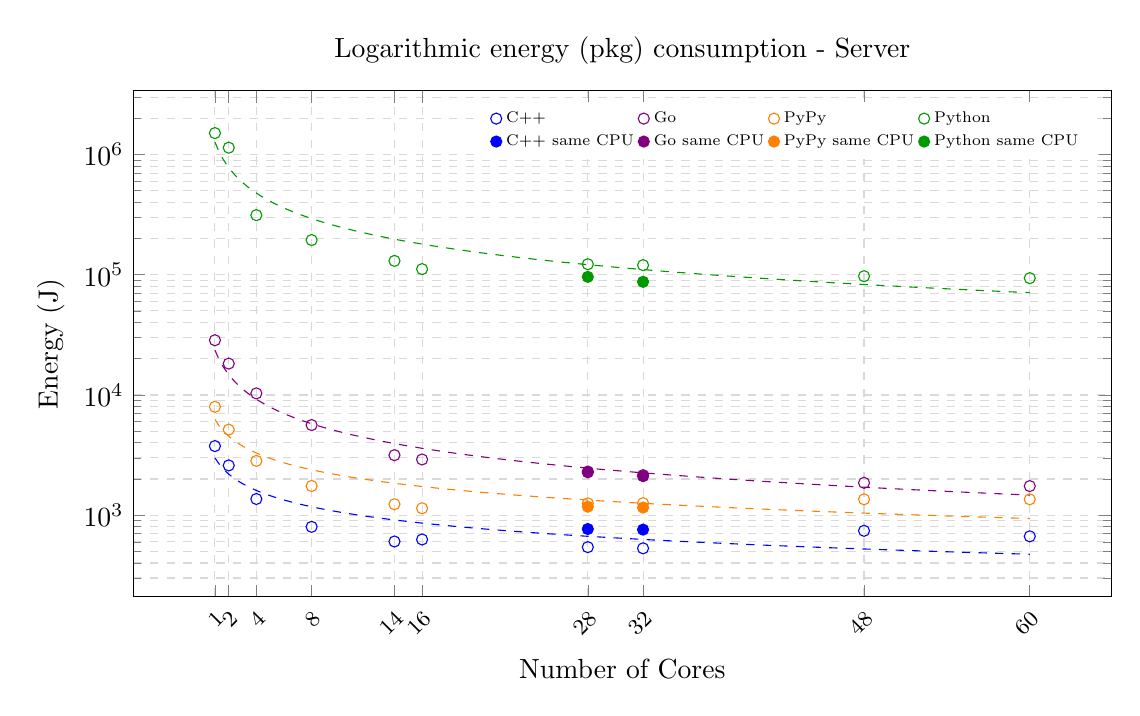
\begin{tikzpicture}
  \begin{semilogyaxis}[
      title={Logarithmic energy (pkg) consumption - Server},
      width=\plotwidthgraph,
      height=\plotheightgraph,
      xlabel={Number of Cores},
      ylabel={Energy (J)},
      ymode=log,
      xmode=linear,
      grid=both,
      minor tick num=1,
      grid style={gray!30,dashed},
      xtick={1,2,4,8,14,16,28,32,48,60},
      x tick label style={
        font=\footnotesize,
        rotate=45,
        anchor=north east
      },
      legend style={
        at={(0.98,0.98)},
        anchor=north east,
        font=\scriptsize,
        nodes={scale=0.8,transform shape},
        draw=none
      },
      legend columns=2,
      transpose legend,
      legend cell align=left,
    ]

    %% C++ %%
    % open circles
    \addplot[
      blue,
      only marks,
      mark=o,
      mark options={draw=blue,fill=white}
    ] table[row sep=\\] {
      x    y \\
      1    3756.26  \\
      2    2591.91  \\
      4    1362.61  \\
      8    799.23   \\
      14   603.37   \\
      16   627.16   \\
      28   541.37   \\  
      32   529.61   \\  
      48   740.57   \\
      60   666.04   \\
    };
    \addlegendentry{C++}
    % filled circles at 28 & 32
    \addplot[
      blue,
      only marks,
      mark=*,
      mark options={draw=blue,fill=blue}
    ] table[row sep=\\] {
      x    y \\
      28   766.51   \\  
      32   757.79   \\  
    };
    \addlegendentry{C++ same CPU}
    % trendline, but do NOT add to legend:
    \addplot[
      blue,
      dashed,
      forget plot,
      domain=1:60,
      samples=200
    ] {3000 * x^(-0.4513)};

    %% Go %%
    \addplot[
      violet,
      only marks,
      mark=o,
      mark options={draw=violet,fill=white}
    ] table[row sep=\\] {
      x    y \\
      1    28522.69 \\
      2    18231.97 \\
      4    10304.27	\\
      8    5617.27  \\
      14   3155.30  \\
      16   2904.52  \\
      28   2306.35  \\
      32   2151.74  \\
      48   1856.93  \\
      60   1744.76  \\
    };
    \addlegendentry{Go}
    \addplot[
      violet,
      only marks,
      mark=*,
      mark options={draw=violet,fill=violet}
    ] table[row sep=\\] {
      x    y \\
      28   2271.71  \\
      32   2109.37  \\
    };
    \addlegendentry{Go same CPU}
    \addplot[
      violet,
      dashed,
      forget plot,
      domain=1:60,
      samples=200
    ] {23600 * x^(-0.6783)};

    %% PyPy %%
    \addplot[
      orange,
      only marks,
      mark=o,
      mark options={draw=orange,fill=white}
    ] table[row sep=\\] {
      x    y \\
      1    7972.65  \\
      2    5147.60  \\
      4    2828.21  \\
      8    1747.96  \\
      14   1232.03  \\
      16   1140.80  \\
      28   1252.93  \\
      32   1257.81  \\
      48   1354.03  \\
      60   1354.03  \\
    };
    \addlegendentry{PyPy}
    \addplot[
      orange,
      only marks,
      mark=*,
      mark options={draw=orange,fill=orange}
    ] table[row sep=\\] {
      x    y \\
      28   1175.52  \\
      32   1155.74  \\
    };
    \addlegendentry{PyPy same CPU}
    \addplot[
      orange,
      dashed,
      forget plot,
      domain=1:60,
      samples=200
    ] {6250 * x^(-0.4633)};

    %% Python %%
    \addplot[
      green!60!black,
      only marks,
      mark=o,
      mark options={draw=green!60!black,fill=white}
    ] table[row sep=\\] {
      x    y \\
      1    1510534.76 \\
      2    1141490.15 \\
      4    313537.85  \\
      8    194458.98  \\
      14   130506.94  \\
      16   111438.01  \\
      28   122384.40  \\
      32   120259.78  \\
      48   97331.00   \\
      60   93718.97   \\
    };
    \addlegendentry{Python}
    \addplot[
      green!60!black,
      only marks,
      mark=*,
      mark options={draw=green!60!black,fill=green!60!black}
    ] table[row sep=\\] {
      x    y \\
      28   96049.86 \\  
      32   87343.61 \\
    };
    \addlegendentry{Python same CPU}
    \addplot[
      green!60!black,
      dashed,
      forget plot,
      domain=1:60,
      samples=200
    ] {1.27e6 * x^(-0.7046)};

  \end{semilogyaxis}
\end{tikzpicture}
\caption{Server - Logarithmic energy (pkg) consumption}{Logarithm energy (pkg) consumption of the Server benchmark across different programming languages.}
\label{fig:log-server-energy-pkg}
\end{figure}


\begin{figure}[h]
  \centering
  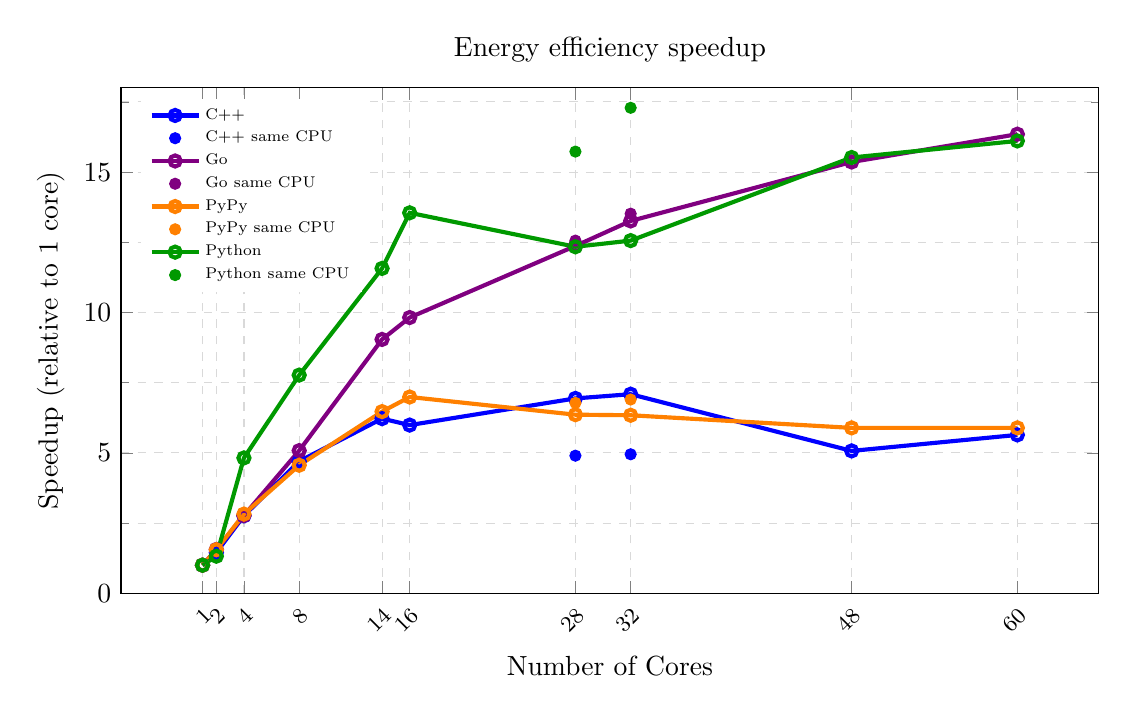
\begin{tikzpicture}
  \begin{axis}[
      title={Energy efficiency speedup},
      width=\plotwidthgraph,
      height=\plotheightgraph,
      xlabel={Number of Cores},
      ylabel={Speedup (relative to 1 core)},
      xmode=linear,
      grid=both,
      minor tick num=1,
      grid style={gray!30,dashed},
      xtick={1,2,4,8,14,16,28,32,48,60},
      x tick label style={
        font=\footnotesize,
        rotate=45,
        anchor=north east
      },
      legend style={
        at={(0.02,0.98)},
        anchor=north west,
        font=\scriptsize,
        nodes={scale=0.8,transform shape},
        draw=none
      },
      legend columns=1,
      legend cell align=left,
      ymin=0,
      ymax=18,
    ]

    %% C++ Speedup (Energy efficiency improvement) %%
    \addplot[
      blue,
      mark=o,
      mark options={draw=blue,fill=white},
      line width=1.5pt
    ] table[row sep=\\] {
      x    y \\
      1    1.00  \\
      2    1.45  \\
      4    2.76  \\
      8    4.70  \\
      14   6.22  \\
      16   5.99  \\
      28   6.94  \\  
      32   7.09  \\  
      48   5.07  \\
      60   5.64  \\
    };
    \addlegendentry{C++}
    
    \addplot[
      blue,
      only marks,
      mark=*,
      mark options={draw=blue,fill=blue}
    ] table[row sep=\\] {
      x    y \\
      28   4.90  \\  
      32   4.95  \\  
    };
    \addlegendentry{C++ same CPU}

    %% Go Speedup %%
    \addplot[
      violet,
      mark=o,
      mark options={draw=violet,fill=white},
      line width=1.5pt
    ] table[row sep=\\] {
      x    y \\
      1    1.00  \\
      2    1.56  \\
      4    2.77  \\
      8    5.08  \\
      14   9.04  \\
      16   9.82  \\
      28   12.37 \\
      32   13.26 \\
      48   15.36 \\
      60   16.35 \\
    };
    \addlegendentry{Go}
    
    \addplot[
      violet,
      only marks,
      mark=*,
      mark options={draw=violet,fill=violet}
    ] table[row sep=\\] {
      x    y \\
      28   12.56 \\
      32   13.52 \\
    };
    \addlegendentry{Go same CPU}

    %% PyPy Speedup %%
    \addplot[
      orange,
      mark=o,
      mark options={draw=orange,fill=white},
      line width=1.5pt
    ] table[row sep=\\] {
      x    y \\
      1    1.00  \\
      2    1.55  \\
      4    2.82  \\
      8    4.56  \\
      14   6.47  \\
      16   6.99  \\
      28   6.36  \\
      32   6.34  \\
      48   5.89  \\
      60   5.89  \\
    };
    \addlegendentry{PyPy}
    
    \addplot[
      orange,
      only marks,
      mark=*,
      mark options={draw=orange,fill=orange}
    ] table[row sep=\\] {
      x    y \\
      28   6.78  \\
      32   6.90  \\
    };
    \addlegendentry{PyPy same CPU}

    %% Python Speedup %%
    \addplot[
      green!60!black,
      mark=o,
      mark options={draw=green!60!black,fill=white},
      line width=1.5pt
    ] table[row sep=\\] {
      x    y \\
      1    1.00  \\
      2    1.32  \\
      4    4.82  \\
      8    7.77  \\
      14   11.57 \\
      16   13.55 \\
      28   12.34 \\
      32   12.56 \\
      48   15.52 \\
      60   16.11 \\
    };
    \addlegendentry{Python}
    
    \addplot[
      green!60!black,
      only marks,
      mark=*,
      mark options={draw=green!60!black,fill=green!60!black}
    ] table[row sep=\\] {
      x    y \\
      28   15.73 \\  
      32   17.29 \\
    };
    \addlegendentry{Python same CPU}

  \end{axis}
  \end{tikzpicture}
\caption{Server - Speedup Energy Efficiency}{Server benchmark energy performance comparison across programming languages: Energy efficiency speedup relative to single-core performance (higher is better).}
\label{fig:energy-comparison}
\end{figure}


\begin{figure}
  \centering
  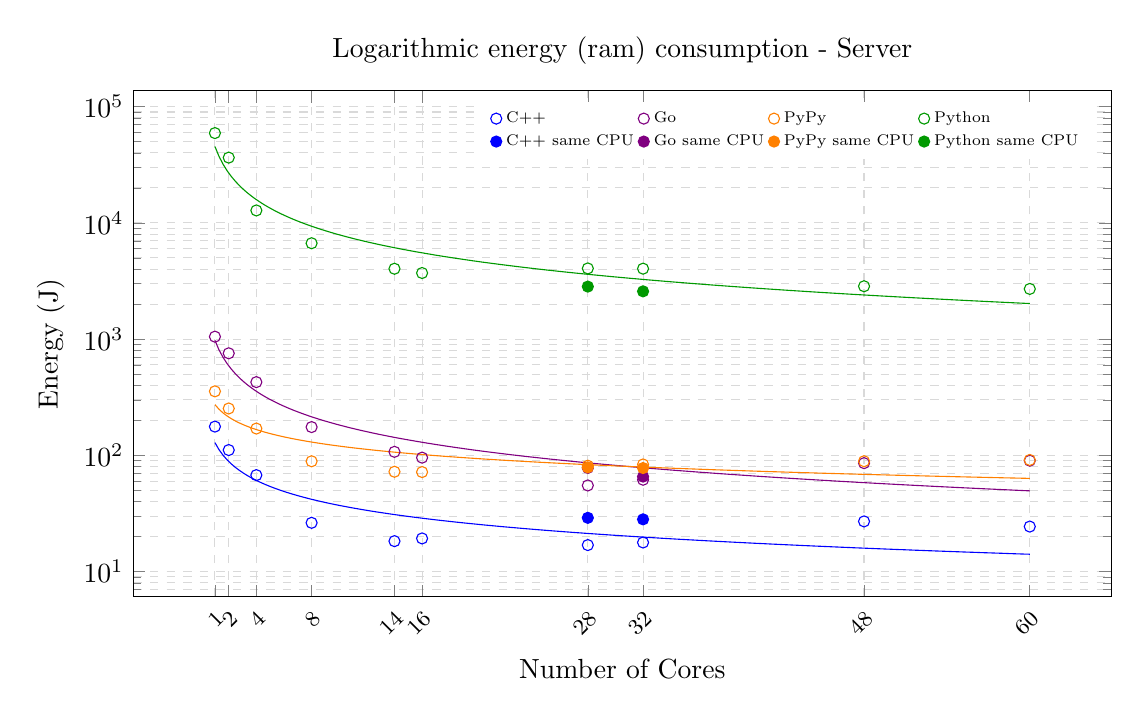
\begin{tikzpicture}
  \begin{semilogyaxis}[
      title={Logarithmic energy (ram) consumption - Server},
      width=\plotwidthgraph,
      height=\plotheightgraph,
      xlabel={Number of Cores},
      ylabel={Energy (J)},
      ymode=log,
      xmode=linear,
      grid=both,
      minor tick num=1,
      grid style={gray!30,dashed},
      xtick={1,2,4,8,14,16,28,32,48,60},
      x tick label style={
        font=\footnotesize,
        rotate=45,
        anchor=north east
      },
      legend style={
        at={(0.98,0.98)},
        anchor=north east,
        font=\scriptsize,
        nodes={scale=0.8,transform shape},
        draw=none
      },
      legend columns=2,
      transpose legend,
      legend cell align=left,
    ]

    %% C++ %%
    \addplot[
      blue,
      only marks,
      mark=o,
      mark options={draw=blue,fill=white}
    ] table[row sep=\\] {
      x    y \\
      1    176.83  \\
      2    111.08  \\
      4    67.60   \\
      8    26.28   \\
      14   18.28   \\
      16   19.29   \\
      28   16.91   \\
      32   17.80   \\
      48   27.02   \\
      60   24.40   \\
    };
    \addlegendentry{C++}
    \addplot[
      blue,
      only marks,
      mark=*,
      mark options={draw=blue,fill=blue}
    ] table[row sep=\\] {
      x    y \\
      28   29.01   \\
      32   28.15   \\
    };
    \addlegendentry{C++ same CPU}
    % power‐law fit: y = 138.9 * x^(–0.5506)
    \addplot[
      blue,
      forget plot,
      domain=1:60,
      samples=200
    ] {128.71 * x^(-0.540)};

    %% Go %%
    \addplot[
      violet,
      only marks,
      mark=o,
      mark options={draw=violet,fill=white}
    ] table[row sep=\\] {
      x    y \\
      1    1049.92 \\
      2    755.43  \\
      4    426.69  \\
      8    175.15  \\
      14   107.26  \\
      16   95.60   \\
      28   55.09   \\
      32   61.70   \\
      48   85.73   \\
      60   90.01   \\
    };
    \addlegendentry{Go}
    \addplot[
      violet,
      only marks,
      mark=*,
      mark options={draw=violet,fill=violet}
    ] table[row sep=\\] {
      x    y \\
      28   78.01   \\
      32   65.66   \\
    };
    \addlegendentry{Go same CPU}
    % power‐law fit: y = 1024.9 * x^(–0.7437)
    \addplot[
      violet,
      forget plot,
      domain=1:60,
      samples=200
    ] {975.38 * x^(-0.728)};

    %% PyPy %%
    \addplot[
      orange,
      only marks,
      mark=o,
      mark options={draw=orange,fill=white}
    ] table[row sep=\\] {
      x    y \\
      1    355.42  \\
      2    253.06  \\
      4    170.08  \\
      8    88.94   \\
      14   72.28   \\
      16   71.84   \\
      28   81.44   \\
      32   83.50   \\
      48   89.06   \\
      60   91.31   \\
    };
    \addlegendentry{PyPy}
    \addplot[
      orange,
      only marks,
      mark=*,
      mark options={draw=orange,fill=orange}
    ] table[row sep=\\] {
      x    y \\
      28   78.81   \\
      32   77.79   \\
    };
    \addlegendentry{PyPy same CPU}
    % power‐law fit: y = 292.4 * x^(–0.3661)
    \addplot[
      orange,
      forget plot,
      domain=1:60,
      samples=200
    ] {273.36 * x^(-0.357)};

    %% Python %%
    \addplot[
      green!60!black,
      only marks,
      mark=o,
      mark options={draw=green!60!black,fill=white}
    ] table[row sep=\\] {
      x    y \\
      1    59269.48 \\
      2    36442.43 \\
      4    12799.44 \\
      8    6683.08  \\
      14   4031.07  \\
      16   3705.32  \\
      28   4057.46  \\
      32   4037.98  \\
      48   2850.62  \\
      60   2703.02  \\
    };
    \addlegendentry{Python}
    \addplot[
      green!60!black,
      only marks,
      mark=*,
      mark options={draw=green!60!black,fill=green!60!black}
    ] table[row sep=\\] {
      x    y \\
      28   2831.52 \\
      32   2576.33 \\
    };
    \addlegendentry{Python same CPU}
    % power‐law fit: y = 4.79e4 * x^(–0.7649)
    \addplot[
      green!60!black,
      forget plot,
      domain=1:60,
      samples=200
    ] {45451.50 * x^(-0.760)};

  \end{semilogyaxis}
\end{tikzpicture}
\caption{Server - Logarithmic energy (ram) consumption}{Logarithm energy (ram) consumption of the Server benchmark across different programming languages.}
\label{fig:log-server-energy-ram}
\end{figure}





\begin{figure}
  \centering

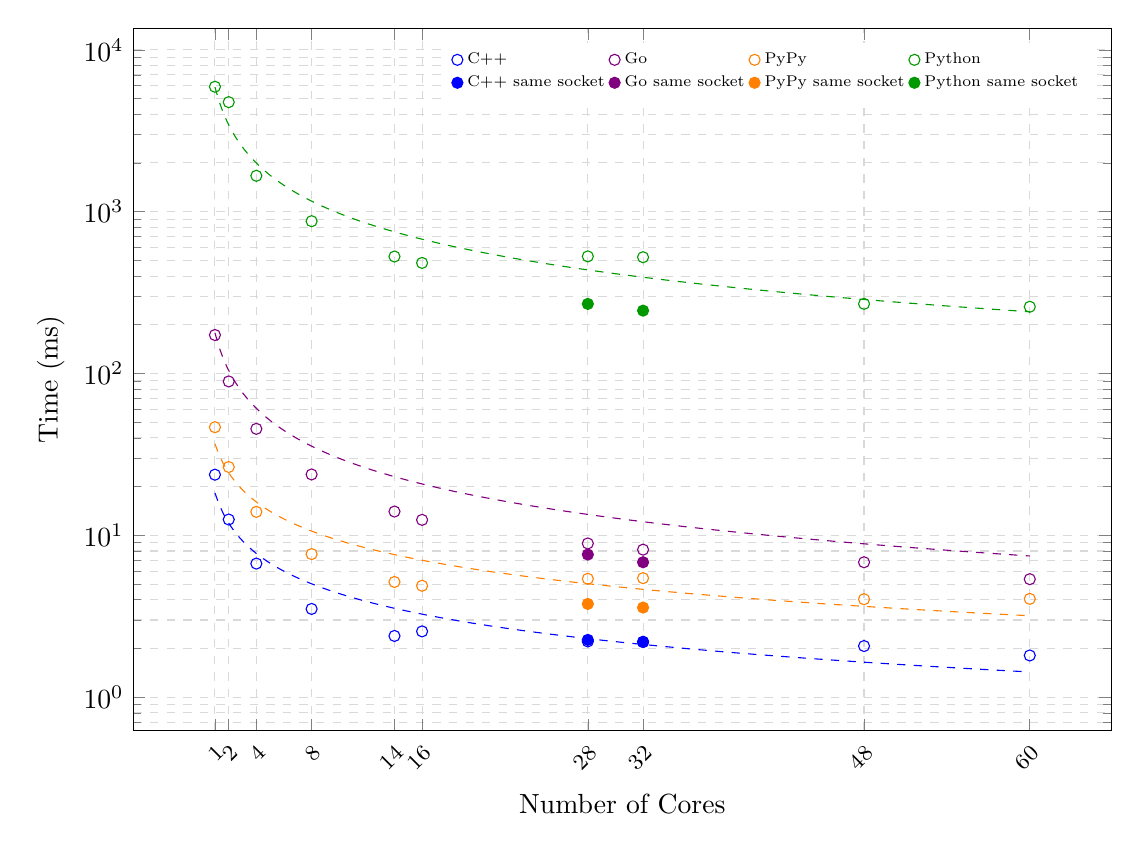
\begin{tikzpicture}
  \begin{semilogyaxis}[
      width=14cm,
      height=10.5cm,
      xlabel={Number of Cores},
      ylabel={Time (ms)},
      ymode=log,
      xmode=linear,
      grid=both,
      minor tick num=1,
      grid style={gray!30,dashed},
      xtick={1,2,4,8,14,16,28,32,48,60},
      x tick label style={
        font=\footnotesize,
        rotate=45,
        anchor=north east
      },
      legend style={
        at={(0.98,0.98)},
        anchor=north east,
        font=\scriptsize,
        nodes={scale=0.8,transform shape},
        draw=none
      },
      legend columns=2,
      transpose legend,
      legend cell align=left,
    ]

    %% C++ %%
    \addplot[
      blue,
      only marks,
      mark=o,
      mark options={draw=blue,fill=white}
    ]
    table[row sep=\\] {
      x    y \\
      1    23.70  \\
      2    12.52  \\
      4    6.69   \\
      8    3.51   \\
      14   2.39   \\
      16   2.55   \\
      28   2.21   \\
      32   2.20   \\
      48   2.07   \\
      60   1.81   \\
    };
    \addlegendentry{C++}

    \addplot[
      blue,
      only marks,
      mark=*,
      mark options={draw=blue,fill=blue}
    ]
    table[row sep=\\] {
      x    y \\
      28   2.26   \\
      32   2.19   \\
    };
    \addlegendentry{C++ same socket}

    % power‐law fit: y = 18.3 * x^(-0.6223)
    \addplot[
      blue,
      dashed,
      forget plot,
      domain=1:60,
      samples=200
    ] {18.3 * x^(-0.6223)};

    %% Go %%
    \addplot[
      violet,
      only marks,
      mark=o,
      mark options={draw=violet,fill=white}
    ]
    table[row sep=\\] {
      x    y \\
      1    172.952 \\
      2    89.32  \\
      4    45.51  \\
      8    23.78  \\
      14   14.03  \\
      16   12.46  \\
      28   8.91   \\
      32   8.16   \\
      48   6.82   \\
      60   5.36   \\
    };
    \addlegendentry{Go}

    \addplot[
      violet,
      only marks,
      mark=*,
      mark options={draw=violet,fill=violet}
    ]
    table[row sep=\\] {
      x    y \\
      28   7.61  \\
      32   6.82  \\
    };
    \addlegendentry{Go same socket}

    % power‐law fit: y = 178.3 * x^(-0.7753)
    \addplot[
      violet,
      dashed,
      forget plot,
      domain=1:60,
      samples=200
    ] {178.3 * x^(-0.7753)};

    %% PyPy %%
    \addplot[
      orange,
      only marks,
      mark=o,
      mark options={draw=orange,fill=white}
    ]
    table[row sep=\\] {
      x    y \\
      1    46.58  \\
      2    26.43  \\
      4    13.97  \\
      8    7.66   \\
      14   5.15   \\
      16   4.88   \\
      28   5.39   \\
      32   5.44   \\
      48   4.03   \\
      60   4.05   \\
    };
    \addlegendentry{PyPy}

    \addplot[
      orange,
      only marks,
      mark=*,
      mark options={draw=orange,fill=orange}
    ]
    table[row sep=\\] {
      x    y \\
      28   3.77   \\
      32   3.58   \\
    };
    \addlegendentry{PyPy same socket}

    % power‐law fit: y = 36.8 * x^(-0.5976)
    \addplot[
      orange,
      dashed,
      forget plot,
      domain=1:60,
      samples=200
    ] {36.8 * x^(-0.5976)};

    %% Python %%
    \addplot[
      green!60!black,
      only marks,
      mark=o,
      mark options={draw=green!60!black,fill=white}
    ]
    table[row sep=\\] {
      x    y \\
      1    5913.41  \\
      2    4749.55  \\
      4    1665.41  \\
      8    872.89   \\
      14   528.12   \\
      16   482.30   \\
      28   529.22   \\
      32   523.04   \\
      48   269.41   \\
      60   258.44   \\
    };
    \addlegendentry{Python}

    \addplot[
      green!60!black,
      only marks,
      mark=*,
      mark options={draw=green!60!black,fill=green!60!black}
    ]
    table[row sep=\\] {
      x    y \\
      28   269.13  \\
      32   244.57  \\
    };
    \addlegendentry{Python same socket}

    % power‐law fit: y = 5894 * x^(-0.7811)
    \addplot[
      green!60!black,
      dashed,
      forget plot,
      domain=1:60,
      samples=200
    ] {5894 * x^(-0.7811)};

  \end{semilogyaxis}
\end{tikzpicture}

\caption{Execution time of the server in Joules for different core configurations}
  \label{fig:server-execution-time}
\end{figure}

\begin{table}[ht]
    \centering
    \begin{tabular}{lrrrr}
        \hline
        time         & C++             & Go            & PyPy          & Python     \\
        \hline
        1            & 23.70           & 172.952       & 46.58         & 5,913.41        \\
        2            & 12.52           & 89.32         & 26.43         & 4,749.55        \\
        4            & 6.69            & 45.51         & 13.97         & 1,665.41        \\
        8	           & 3.51  	         & 23.78 	       & 7.66          & 872.89          \\
        14           & 2.39            & 14.03         & 5.15          & 528.12          \\
        16           & 2.55            & 12.46         & 4.88          & 482.30          \\
        28           & 2.21            & 8.91          & 5.39          & 529.22          \\
        28 same CPU  & 2.26            & 7.61          & 3.77          & 269.13          \\
        32           & 2.20            & 8.16          & 5.44          & 523.04          \\
        32 same CPU  & 2.19            & 6.82          & 3.58          & \textbf{244.57} \\
        48           & 2.07            & 6.82          & 4.03          & 269.41          \\
        60           & \textbf{1.81}   & \textbf{5.36} & \textbf{4.05} & 258.44          \\
        \hline
    \end{tabular}
    \caption{Execution time by implementation and core count}
    \label{tab:server-execution-time}
\end{table}

\begin{figure}
    \centering
    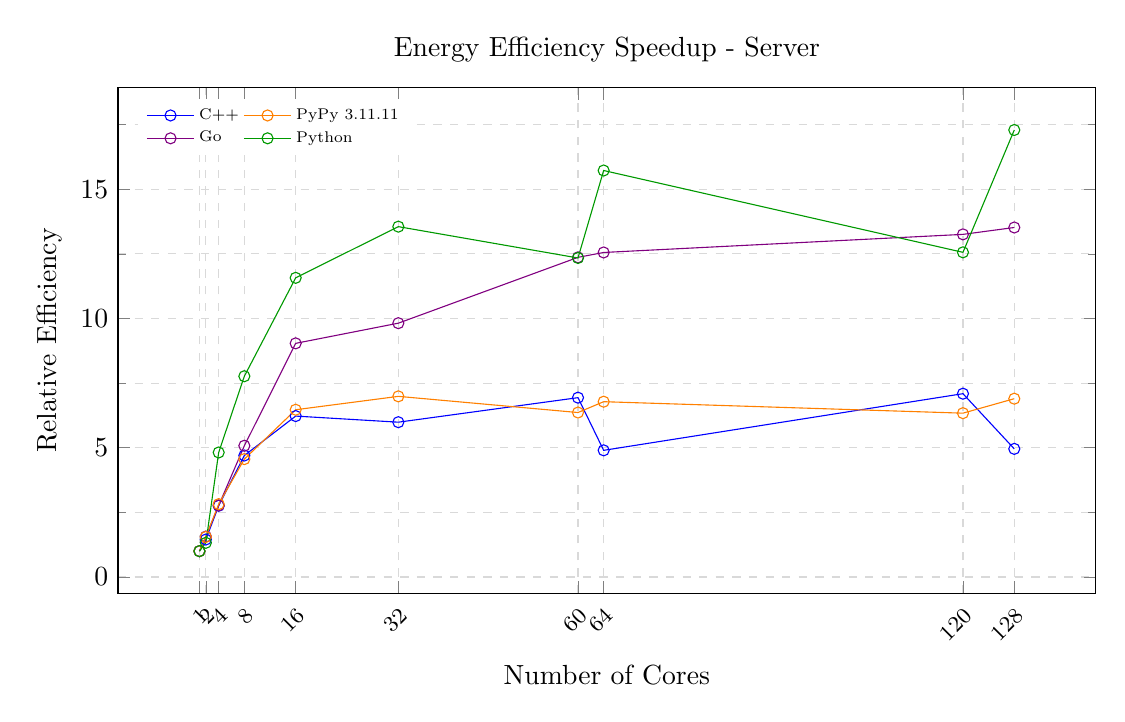
\begin{tikzpicture}
  \begin{axis}[
      title={Energy Efficiency Speedup - Server},
      width=\plotwidthgraph,
      height=\plotheightgraph,
      xlabel={Number of Cores},
      ylabel={Relative Efficiency},
      ymode=linear,
      xmode=linear,
      grid=both,
      minor tick num=1,
      grid style={gray!30,dashed},
      xtick={1,2,4,8,16,32,60,64,120,128},
      x tick label style={
        font=\footnotesize,
        rotate=45,
        anchor=north east
      },
      legend style={
        at={(0.02,0.98)},
        anchor=north west,
        font=\scriptsize,
        nodes={scale=0.8,transform shape},
        draw=none
      },
      legend columns=2,
      transpose legend,
      legend cell align=left,
    ]
    %% C++ %%
    \addplot[
      blue,
      mark=o,
    ]
    table[row sep=\\] {
      x   y     \\
      1   1 \\
      2   1.449224703 \\
      4   2.756665517 \\
      8   4.699848604 \\
      16  6.225466961 \\
      32  5.989316921 \\
      60  6.938433973 \\
      64  4.900470966 \\
      120 7.09250203 \\
      128 4.9568614 \\
    };
    \addlegendentry{C++}

    %% Go %%
    \addplot[
      violet,
      mark=o,
    ]
    table[row sep=\\] {
      x   y     \\
      1   1 \\
      2   1.564432697 \\
      4   2.768045674 \\
      8   5.077678303 \\
      16  9.039612715 \\
      32  9.820104527 \\
      60  12.36702582 \\
      64  12.55560349 \\
      120 13.25563962 \\
      128 13.5218999 \\
    };
    \addlegendentry{Go}

    %% PyPy 3.11.11 %%
    \addplot[
      orange,
      mark=o,
    ]
    table[row sep=\\] {
      x   y     \\
      1   1 \\
      2   1.548809154 \\
      4   2.818973839 \\
      8   4.561116959 \\
      16  6.471149241 \\
      32  6.988648317 \\
      60  6.363204648 \\
      64  6.782232544 \\
      120 6.338516946 \\
      128 6.898307578 \\
    };
    \addlegendentry{PyPy 3.11.11}

    %% Python %%
    \addplot[
      green!60!black,
      mark=o,
    ]
    table[row sep=\\] {
      x   y     \\
      1   1 \\
      2   1.323300741 \\
      4   4.817711048 \\
      8   7.767883818 \\
      16  11.57436351 \\
      32  13.55493304 \\
      60  12.34254336 \\
      64  15.72656914 \\
      120 12.5605981 \\
      128 17.29416455 \\
    };
    \addlegendentry{Python}

  \end{axis}
\end{tikzpicture}
    \caption{Server - Energy Efficiency Speedup}{Energy efficiency speedup of the Server benchmark across different programming languages.}
    \label{fig:server-speedup}
\end{figure}



From \autoref{fig:log-server-energy-pkg}, we can see that the energy consumption of the server is not linear with the number of cores. It can be observed that the energy consumption decreases as the number of cores increases, but there is a point in the graph and \autoref{tab:server-energy-pkg} where the energy consumption starts to increase slightly again, as well as the execution times in \autoref{fig:log-server-execution-time}, but not as much as the energy consumption.

This is due to hyperthreading \footnote{Hyperthreading is enabled in this system. To set the process to a fixed \gls{cpu}, I used \texttt{taskset -c [cores]}, i.e., \texttt{taskset -c 0-15,32-47} for running across multiple \glspl{cpu} and \texttt{taskset -c 0-31} to force the program to only run in a single \gls{cpu}.} in the \glspl{cpu}, which allows the \glspl{cpu} to run two threads per core, but this is not as efficient as running a single thread per core, as the \glspl{cpu} have to share resources between the two threads.

It is obvious from the multiple graphs and tables that the C++ implementation is the most energy-efficient and fastest by a significant margin, followed surprisingly by the PyPy execution of the Python code, which is faster than the Go implementation, and the Python implementation is the slowest and most energy-consuming by an extremely large amount.

However, when looking closely at the 28-core and 32-core tests, focusing on C++, we can see the energy consumption is lower when using cores from different CPUs rather than consuming more, as there is some energy efficiency loss when synchronizing the data between the two CPUs. What happens in this case is that the C++ parallelization algorithm makes each of the cores have a very hard \gls{cpu} workload, resulting in a more efficient result. This aligns with \autoref{sec:hyperthreading}, where it is explained that hyperthreading is not as efficient for specific tasks.

I want to specifically discuss the 60-core test, as it is the most interesting one. In this test, the energy consumption is lower than in the 48-core test, as well as the execution time on the C++ implementation, but on the Go implementation, both energy consumption and execution time are higher than in the 48-core test. This is because the Go implementation is not as efficient as the C++ implementation, and the Go runtime has to manage more goroutines, which adds overhead.

Considering the 32-core and 48-core tests with the Python program, the energy consumption reduces significantly when the program starts using virtual cores, as the program is able to run on more cores, and the Python runtime is not very demanding, being able to use these cores efficiently. As shown in \autoref{fig:log-server-energy-pkg} and \autoref{fig:log-server-execution-time}, this is an advantage to Python with respect to itself.


A usually not looked aspect is the energy consumed by the \gls{ram} in the system, which is shown in \autoref{fig:log-server-energy-ram}. As we can see, the energy consumed by the \gls{ram} is not linear with the number of cores, and after incrementing the cores to more than $8$ cores, the energy consumption does not decrease substantially. But we can see that when using the cores in the same processor, (28 same CPU \& 32 same CPU), the RAM energy consumption is much higher than their counterpart using different processors when using \textbf{C++} or \textbf{Go}. But, at those same core counts, if we check the \textbf{Python} and \textbf{PyPy} implementations, the energy consumption is lower when using the same processor, as the Python runtime is not very demanding and does not require much memory bandwidth, thus being able to use the memory more efficiently.



\begin{figure}
    \centering
    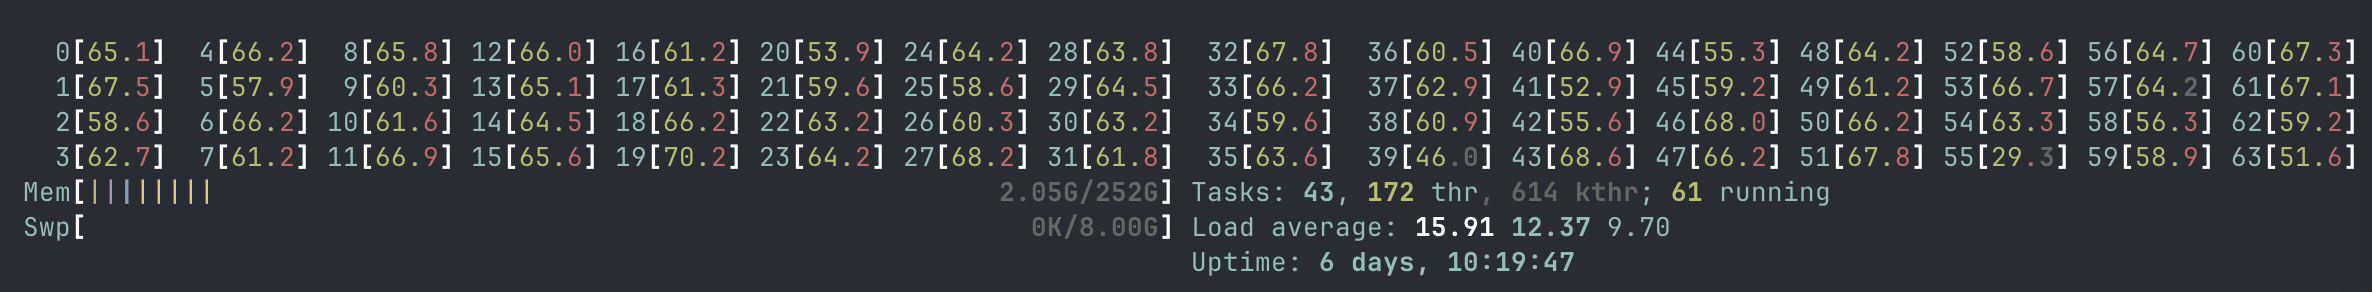
\includegraphics[width=1\linewidth]{img/htop_not_running_100_60_cores.png}
    \caption[Core usage per pixel renderer]{\gls{htop} showing the cores not being used at 100\% when using many cores for processing in a per-pixel multi threading renderer }
    \label{fig:htop_60_not_100}
\end{figure}

It also must be noted that the cores during the 48 core benchmark were being used at 100\% of their capacity, while in the 60 cores test, the cores were mostly being used at a lower percentage, as shown in \autoref{fig:htop_60_not_100}. This is because the Go runtime is not able to efficiently use all the cores when there are more than 48 cores available, and it is not able to schedule the goroutines efficiently as these routines finish so fast that the Go runtime is not able to keep all the cores busy.

If we changed the implementation to a per-row renderer, on the go-side, the Go runtime would be able to use all the cores more efficiently, as it would be able to schedule the goroutines more efficiently, and the execution time would be lower, but the energy consumption would be higher, as the cores would be used at 100\% of their capacity. Thus, in this case, as we will see in other sections, having a faster execution time is not always the best option in terms of energy consumption.


All the raw data for the benchmarks can be found in the \autoref{chap:appendix-server-benchmarks}.

% When changin to a per-pixel rendered, lower cores energy efficiency increased, but the many cores, from 48 oward would not get used as much, thus reducing the energy efficiency and increating the execution time. 



\subsection{Desktop}
This platform is one of the most common in the amateur market, as it is a personal desktop computer with a Ryzen 3800x processor, which has 8 cores and 16 threads and has 32GB of RAM. It has a Zen 2 architecture, which has heterogeneous cores. These tests were performed with hyperthreading enabled, as it is the most popular configuration, and the default configuration. 

\subsubsection{Cache \& Numa}
The cache of the AMD Ryzen 3800x is shown in \autoref{lst:ryzen-cache}. As we can see, it has 8 instances of 256 KiB of L1 data cache and 256 KiB of L1 instruction cache, which is half the number of threads available in the system (the same as the server platform). It has also two L3 caches of 32 MiB each, which is due to the processor having two \glspl{CCX}. 

\begin{lstlisting}[language=bash, caption={Cache of the AMD Ryzen 3800x}, label={lst:ryzen-cache}]
  $ lscpu | grep -i cache
  Caches (sum of all):
    L1d:                    256 KiB (8 instances)
    L1i:                    256 KiB (8 instances)
    L2:                     4 MiB (8 instances)
    L3:                     32 MiB (2 instances)
  NUMA:
    NUMA node(s):           1
    NUMA node0 CPU(s):      0-7
  \end{lstlisting}


\subsubsection{Results}

\begin{figure}
    \centering
    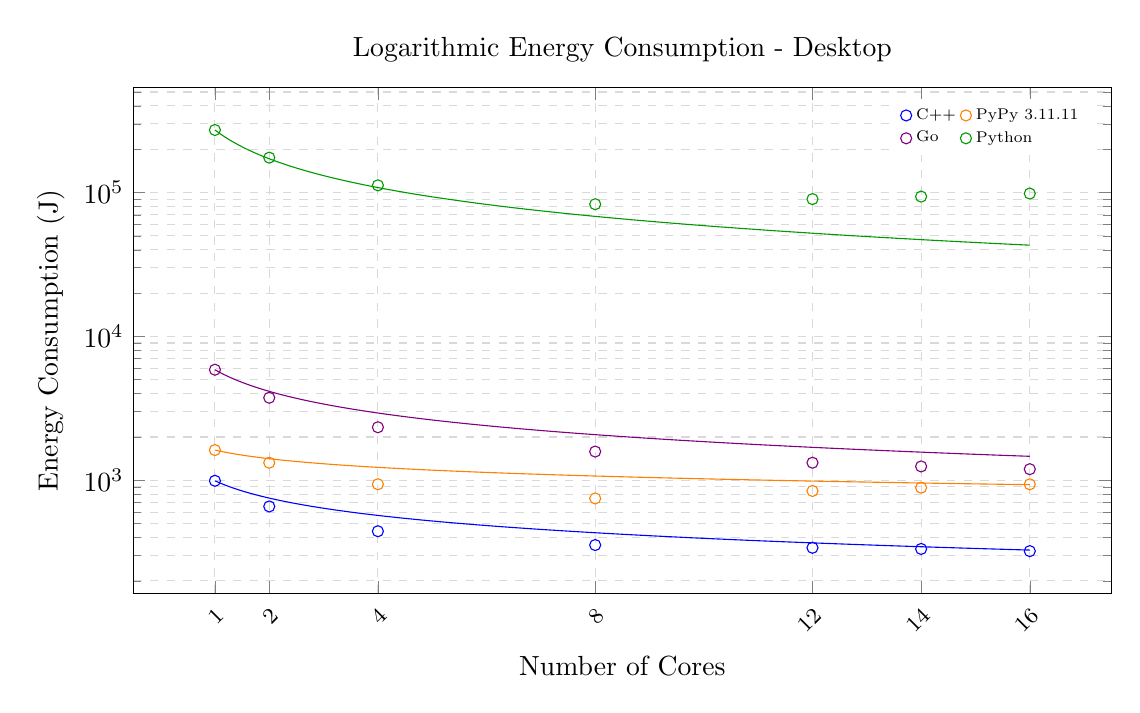
\begin{tikzpicture}
  \begin{semilogyaxis}[
      title={Logarithmic Energy Consumption - Desktop},
      width=\plotwidthgraph,
      height=\plotheightgraph,
      xlabel={Number of Cores},
      ylabel={Energy Consumption (J)},
      ymode=log,
      xmode=linear,
      grid=both,
      minor tick num=1,
      grid style={gray!30,dashed},
      xtick={1,2,4,8,12,14,16},
      x tick label style={
        font=\footnotesize,
        rotate=45,
        anchor=north east
      },
      legend style={
        at={(0.98,0.98)},
        anchor=north east,
        font=\scriptsize,
        nodes={scale=0.8,transform shape},
        draw=none
      },
      legend columns=2,
      transpose legend,
      legend cell align=left,
    ]
    %% C++ %%
    \addplot[
      blue,
      only marks,
      mark=o,
      mark options={draw=blue,fill=white}
    ]
    table[row sep=\\] {
      x   y      \\
      1   991.49 \\
      2   657.79 \\
      4   442.17 \\
      8   354.57 \\
      12  339.44 \\
      14  333.01 \\
      16  321.60 \\
    };
    \addlegendentry{C++}
    % power-law fit: y = 991.49 * x^(-0.4)
    \addplot[
      blue,
      forget plot,
      domain=1:16,
      samples=200
    ] {991.49 * x^(-0.4)};

    %% Go %%
    \addplot[
      violet,
      only marks,
      mark=o,
      mark options={draw=violet,fill=white}
    ]
    table[row sep=\\] {
      x   y       \\
      1   5867.26 \\
      2   3746.84 \\
      4   2335.54 \\
      8   1583.17 \\
      12  1324.22 \\
      14  1247.80 \\
      16  1194.03 \\
    };
    \addlegendentry{Go}
    % power-law fit: y = 5867.26 * x^(-0.5)
    \addplot[
      violet,
      forget plot,
      domain=1:16,
      samples=200
    ] {5867.26 * x^(-0.5)};

    %% PyPy 3.11.11 %%
    \addplot[
      orange,
      only marks,
      mark=o,
      mark options={draw=orange,fill=white}
    ]
    table[row sep=\\] {
      x   y       \\
      1   1621.77 \\
      2   1324.05 \\
      4   938.02  \\
      8   747.41  \\
      12  842.68  \\
      14  889.03  \\
      16  937.02  \\
    };
    \addlegendentry{PyPy 3.11.11}
    % power-law fit: y = 1621.77 * x^(-0.2)
    \addplot[
      orange,
      forget plot,
      domain=1:16,
      samples=200
    ] {1621.77 * x^(-0.2)};

    %% Python %%
    \addplot[
      green!60!black,
      only marks,
      mark=o,
      mark options={draw=green!60!black,fill=white}
    ]
    table[row sep=\\] {
      x    y         \\
      1    272235.58 \\
      2    174822.21 \\
      4    112247.92 \\
      8    82983.52  \\
      12   90069.44  \\
      14   93771.09  \\
      16   98436.51  \\
    };
    \addlegendentry{Python}
    % power-law fit: y = 272235.58 * x^(-0.665)
    \addplot[
      green!60!black,
      forget plot,
      domain=1:16,
      samples=200
    ] {272235.58 * x^(-0.665)};

  \end{semilogyaxis}
\end{tikzpicture}
    \caption{Desktop - Logarithmic energy consumption}{Logarithm energy consumption of the Desktop benchmark across different programming languages}
    \label{fig:log-desktop-energy}
\end{figure}

\begin{figure}
    \centering
    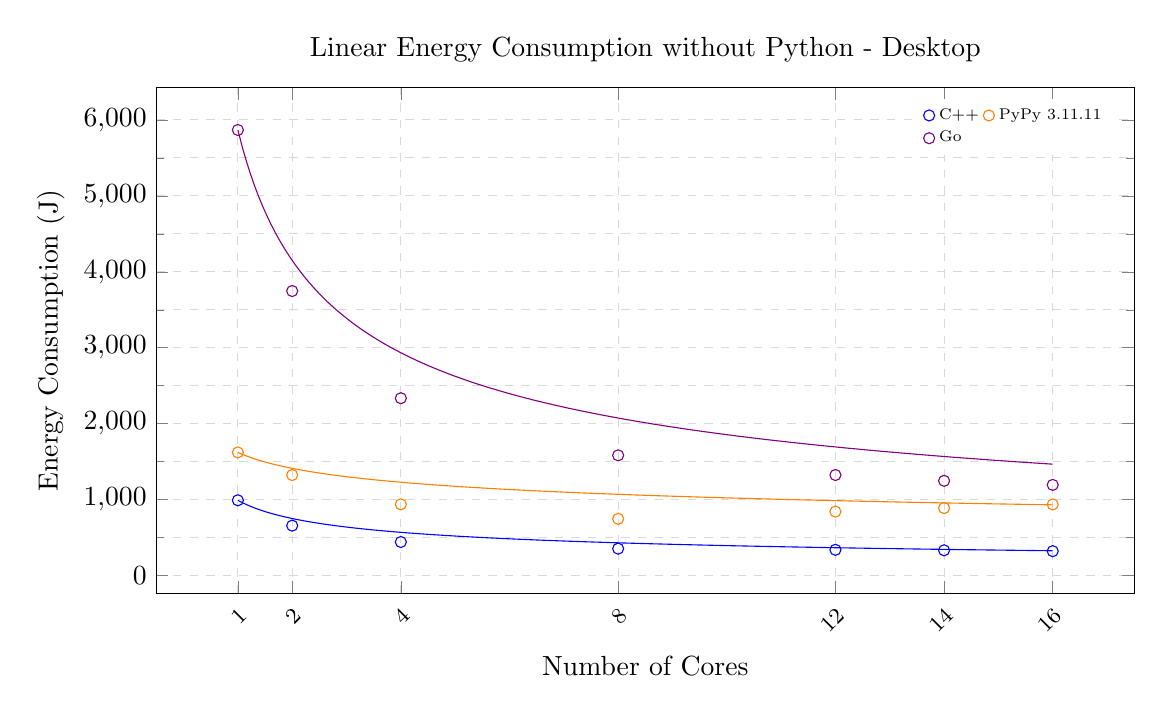
\begin{tikzpicture}
  \begin{axis}[
      title={Linear Energy Consumption without Python - Desktop},
      width=\plotwidthgraph,
      height=\plotheightgraph,
      xlabel={Number of Cores},
      ylabel={Energy Consumption (J)},
      ymode=linear,
      xmode=linear,
      grid=both,
      minor tick num=1,
      grid style={gray!30,dashed},
      xtick={1,2,4,8,12,14,16},
      x tick label style={
        font=\footnotesize,
        rotate=45,
        anchor=north east
      },
      legend style={
        at={(0.98,0.98)},
        anchor=north east,
        font=\scriptsize,
        nodes={scale=0.8,transform shape},
        draw=none
      },
      legend columns=2,
      transpose legend,
      legend cell align=left,
    ]
    %% C++ %%
    \addplot[
      blue,
      only marks,
      mark=o,
      mark options={draw=blue,fill=white}
    ]
    table[row sep=\\] {
      x   y      \\
      1   991.49 \\
      2   657.79 \\
      4   442.17 \\
      8   354.57 \\
      12  339.44 \\
      14  333.01 \\
      16  321.60 \\
    };
    \addlegendentry{C++}
    % power-law fit: y = 991.49 * x^(-0.4)
    \addplot[
      blue,
      forget plot,
      domain=1:16,
      samples=200
    ] {991.49 * x^(-0.4)};

    %% Go %%
    \addplot[
      violet,
      only marks,
      mark=o,
      mark options={draw=violet,fill=white}
    ]
    table[row sep=\\] {
      x   y       \\
      1   5867.26 \\
      2   3746.84 \\
      4   2335.54 \\
      8   1583.17 \\
      12  1324.22 \\
      14  1247.80 \\
      16  1194.03 \\
    };
    \addlegendentry{Go}
    % power-law fit: y = 5867.26 * x^(-0.5)
    \addplot[
      violet,
      forget plot,
      domain=1:16,
      samples=200
    ] {5867.26 * x^(-0.5)};

    %% PyPy 3.11.11 %%
    \addplot[
      orange,
      only marks,
      mark=o,
      mark options={draw=orange,fill=white}
    ]
    table[row sep=\\] {
      x   y       \\
      1   1621.77 \\
      2   1324.05 \\
      4   938.02  \\
      8   747.41  \\
      12  842.68  \\
      14  889.03  \\
      16  937.02  \\
    };
    \addlegendentry{PyPy 3.11.11}
    % power-law fit: y = 1621.77 * x^(-0.2)
    \addplot[
      orange,
      forget plot,
      domain=1:16,
      samples=200
    ] {1621.77 * x^(-0.2)};

  \end{axis}
\end{tikzpicture}
    \caption{Desktop - Linear energy consumption}{Linear energy consumption of the Desktop benchmark across different programming languages}
    \label{fig:linear-desktop-energy-hyperthreading}
\end{figure}


\begin{figure}
    \centering
    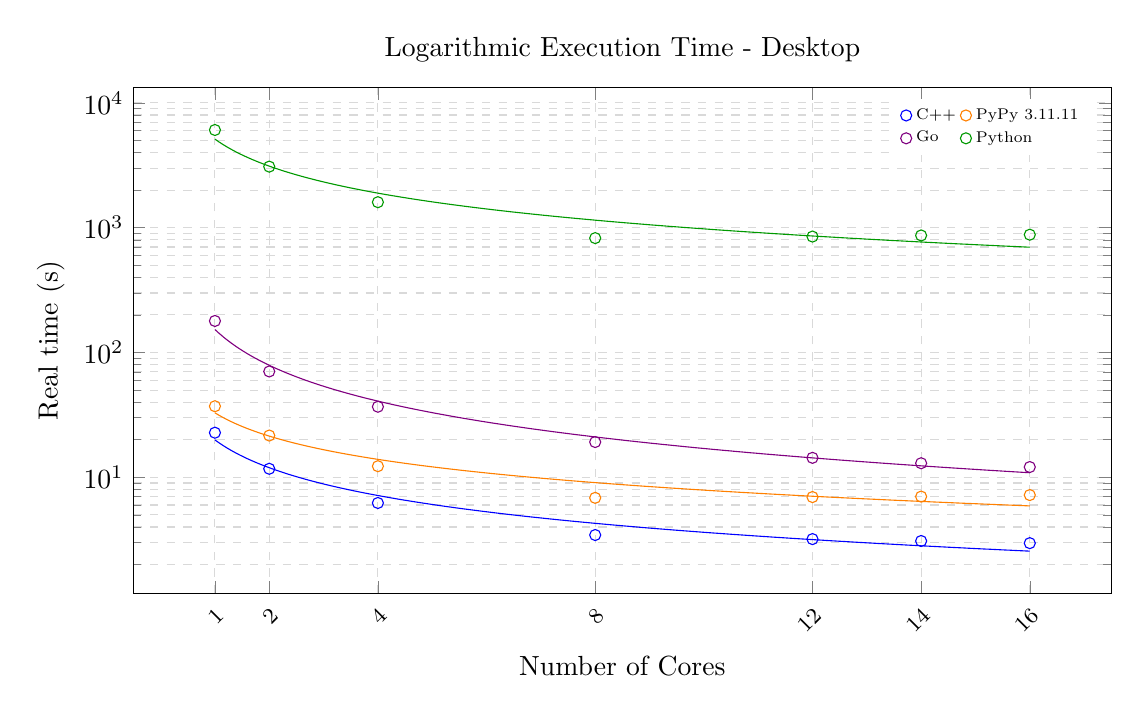
\begin{tikzpicture}
  \begin{semilogyaxis}[
      title={Logarithmic Execution Time - Desktop},
      width=\plotwidthgraph,
      height=\plotheightgraph,
      xlabel={Number of Cores},
      ylabel={Real time (s)},
      ymode=log,
      xmode=linear,
      grid=both,
      minor tick num=1,
      grid style={gray!30,dashed},
      xtick={1,2,4,8,12,14,16},
      x tick label style={
        font=\footnotesize,
        rotate=45,
        anchor=north east
      },
      legend style={
        at={(0.98,0.98)},
        anchor=north east,
        font=\scriptsize,
        nodes={scale=0.8,transform shape},
        draw=none
      },
      legend columns=2,
      transpose legend,
      legend cell align=left,
    ]
    %% C++ %%
    \addplot[
      blue,
      only marks,
      mark=o,
      mark options={draw=blue,fill=white}
    ]
    table[row sep=\\] {
      x   y     \\
      1   22.78 \\
      2   11.71 \\
      4   6.23  \\
      8   3.45  \\
      12  3.20  \\
      14  3.09  \\
      16  2.97  \\
    };
    \addlegendentry{C++}
    % power-law fit: y = 22.78 * x^(-0.8)
    \addplot[
      blue,
      forget plot,
      domain=1:16,
      samples=200
    ] {19.94 * x^(-0.740)};

    %% Go %%
    \addplot[
      violet,
      only marks,
      mark=o,
      mark options={draw=violet,fill=white}
    ]
    table[row sep=\\] {
      x   y      \\
      1   178.98 \\
      2   70.51  \\
      4   36.79  \\
      8   19.18  \\
      12  14.33  \\
      14  12.97  \\
      16  12.09  \\
    };
    \addlegendentry{Go}
    % power-law fit: y = 178.98 * x^(-0.9)
    \addplot[
      violet,
      forget plot,
      domain=1:16,
      samples=200
    ] {152.85 * x^(-0.953)};

    %% PyPy 3.11.11 %%
    \addplot[
      orange,
      only marks,
      mark=o,
      mark options={draw=orange,fill=white}
    ]
    table[row sep=\\] {
      x   y      \\
      1   37.12  \\
      2   21.62  \\
      4   12.28  \\
      8   6.85   \\
      12  6.95   \\
      14  7.01   \\
      16  7.21   \\
    };
    \addlegendentry{PyPy 3.11.11}
    % power-law fit: y = 37.12 * x^(-0.7)
    \addplot[
      orange,
      forget plot,
      domain=1:16,
      samples=200
    ] {32.85 * x^(-0.619)};

    %% Python %%
    \addplot[
      green!60!black,
      only marks,
      mark=o,
      mark options={draw=green!60!black,fill=white}
    ]
    table[row sep=\\] {
      x    y       \\
      1    6063.96 \\
      2    3084.07 \\
      4    1600.72 \\
      8    825.24  \\
      12   848.99  \\
      14   866.47  \\
      16   878.90  \\
    };
    \addlegendentry{Python}
    % power-law fit: y = 6063.96 * x^(-0.870)
    \addplot[
      green!60!black,
      forget plot,
      domain=1:16,
      samples=200
    ] {5123.25 * x^(-0.719)};

  \end{semilogyaxis}
\end{tikzpicture}
    \caption{Desktop - Logarithmic Execution Time}{Logarithm Execution time of the Desktop benchmark across different programming languages.}
    \label{fig:log-desktop-execution-time}
    
\end{figure}

\begin{figure}
    \centering
    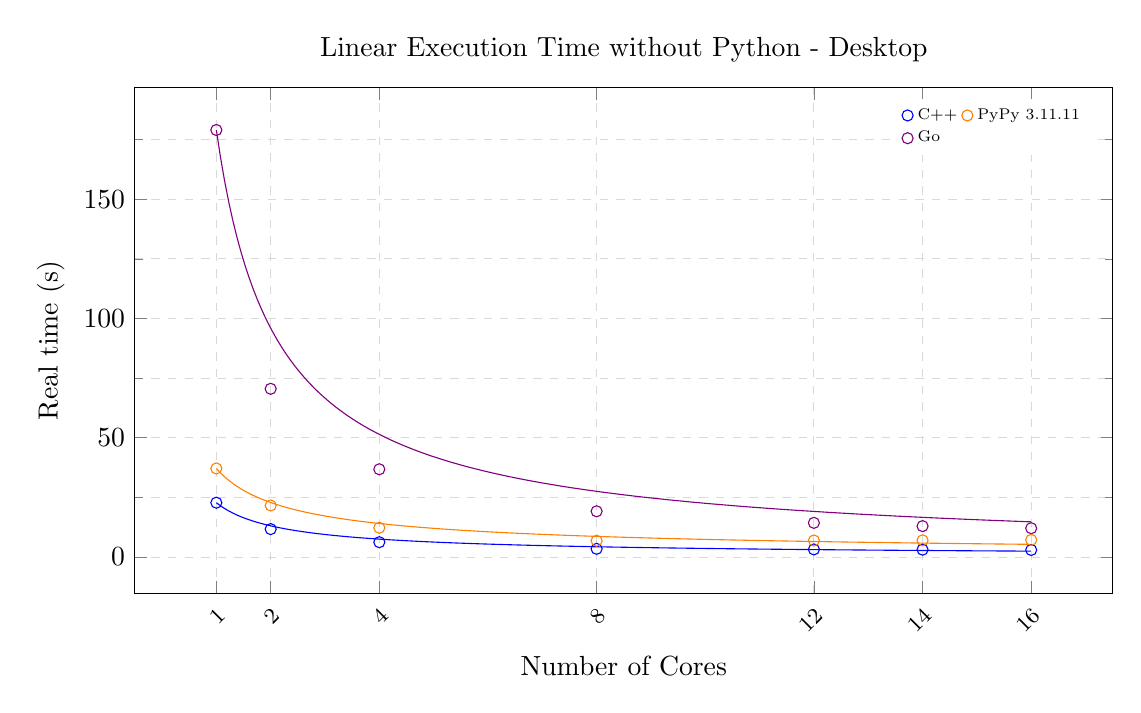
\begin{tikzpicture}
  \begin{axis}[
      title={Linear Execution Time without Python - Desktop},
      width=\plotwidthgraph,
      height=\plotheightgraph,
      xlabel={Number of Cores},
      ylabel={Real time (s)},
      ymode=linear,
      xmode=linear,
      grid=both,
      minor tick num=1,
      grid style={gray!30,dashed},
      xtick={1,2,4,8,12,14,16},
      x tick label style={
        font=\footnotesize,
        rotate=45,
        anchor=north east
      },
      legend style={
        at={(0.98,0.98)},
        anchor=north east,
        font=\scriptsize,
        nodes={scale=0.8,transform shape},
        draw=none
      },
      legend columns=2,
      transpose legend,
      legend cell align=left,
    ]
    %% C++ %%
    \addplot[
      blue,
      only marks,
      mark=o,
      mark options={draw=blue,fill=white}
    ]
    table[row sep=\\] {
      x   y     \\
      1   22.78 \\
      2   11.71 \\
      4   6.23  \\
      8   3.45  \\
      12  3.20  \\
      14  3.09  \\
      16  2.97  \\
    };
    \addlegendentry{C++}
    % power-law fit: y = 22.78 * x^(-0.8)
    \addplot[
      blue,
      forget plot,
      domain=1:16,
      samples=200
    ] {22.78 * x^(-0.8)};

    %% Go %%
    \addplot[
      violet,
      only marks,
      mark=o,
      mark options={draw=violet,fill=white}
    ]
    table[row sep=\\] {
      x   y      \\
      1   178.98 \\
      2   70.51  \\
      4   36.79  \\
      8   19.18  \\
      12  14.33  \\
      14  12.97  \\
      16  12.09  \\
    };
    \addlegendentry{Go}
    % power-law fit: y = 178.98 * x^(-0.9)
    \addplot[
      violet,
      forget plot,
      domain=1:16,
      samples=200
    ] {178.98 * x^(-0.9)};

    %% PyPy 3.11.11 %%
    \addplot[
      orange,
      only marks,
      mark=o,
      mark options={draw=orange,fill=white}
    ]
    table[row sep=\\] {
      x   y      \\
      1   37.12  \\
      2   21.62  \\
      4   12.28  \\
      8   6.85   \\
      12  6.95   \\
      14  7.01   \\
      16  7.21   \\
    };
    \addlegendentry{PyPy 3.11.11}
    % power-law fit: y = 37.12 * x^(-0.7)
    \addplot[
      orange,
      forget plot,
      domain=1:16,
      samples=200
    ] {37.12 * x^(-0.7)};

  \end{axis}
\end{tikzpicture}
    \caption{Desktop - Linear execution Time}{Linear execution time of the laptop benchmark across different programming languages without Python.}
    \label{fig:linear-desktop-execution-time-hyperthreading}
\end{figure}


\begin{figure}
    \centering
    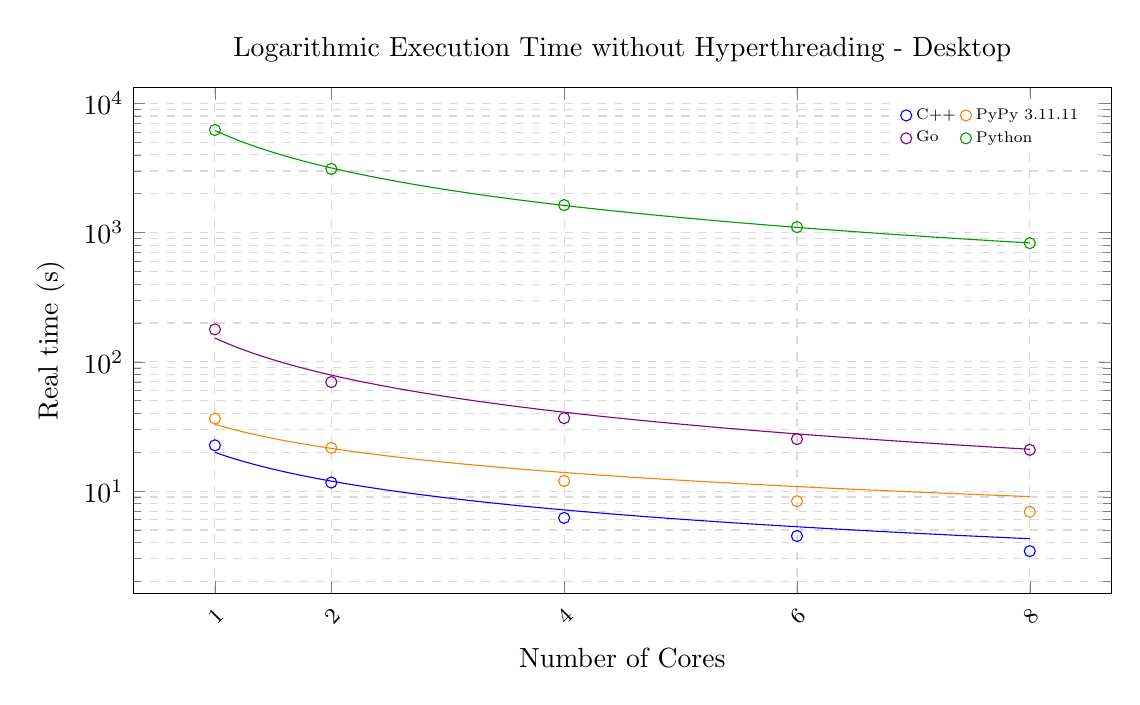
\begin{tikzpicture}
  \begin{semilogyaxis}[
      title={Logarithmic Execution Time without Hyperthreading - Desktop},
      width=\plotwidthgraph,
      height=\plotheightgraph,
      xlabel={Number of Cores},
      ylabel={Real time (s)},
      ymode=log,
      xmode=linear,
      grid=both,
      minor tick num=1,
      grid style={gray!30,dashed},
      xtick={1,2,4,6,8},
      x tick label style={
        font=\footnotesize,
        rotate=45,
        anchor=north east
      },
      legend style={
        at={(0.98,0.98)},
        anchor=north east,
        font=\scriptsize,
        nodes={scale=0.8,transform shape},
        draw=none
      },
      legend columns=2,
      transpose legend,
      legend cell align=left,
    ]
    %% C++ %%
    \addplot[
      blue,
      only marks,
      mark=o,
      mark options={draw=blue,fill=white}
    ]
    table[row sep=\\] {
      x   y     \\
      1   22.60 \\
      2   11.64 \\
      4   6.20  \\
      6   4.49  \\
      8   3.43  \\
    };
    \addlegendentry{C++}
    % power-law fit: y = 22.60 * x^(-0.8)
    \addplot[
      blue,
      forget plot,
      domain=1:8,
      samples=200
    ] {19.94 * x^(-0.740)};

    %% Go %%
    \addplot[
      violet,
      only marks,
      mark=o,
      mark options={draw=violet,fill=white}
    ]
    table[row sep=\\] {
      x   y      \\
      1   178.43 \\
      2   69.77  \\
      4   36.68  \\
      6   25.24  \\
      8   20.84  \\
    };
    \addlegendentry{Go}
    % power-law fit: y = 178.43 * x^(-0.9)
    \addplot[
      violet,
      forget plot,
      domain=1:8,
      samples=200
    ] {152.85 * x^(-0.953)};

    %% PyPy 3.11.11 %%
    \addplot[
      orange,
      only marks,
      mark=o,
      mark options={draw=orange,fill=white}
    ]
    table[row sep=\\] {
      x   y      \\
      1   36.42  \\
      2   21.59  \\
      4   11.97  \\
      6   8.35   \\
      8   6.91   \\
    };
    \addlegendentry{PyPy 3.11.11}
    % power-law fit: y = 36.42 * x^(-0.7)
    \addplot[
      orange,
      forget plot,
      domain=1:8,
      samples=200
    ] {32.85 * x^(-0.619)};

    %% Python %%
    \addplot[
      green!60!black,
      only marks,
      mark=o,
      mark options={draw=green!60!black,fill=white}
    ]
    table[row sep=\\] {
      x    y       \\
      1    6232.49 \\
      2    3115.45 \\
      4    1634.00 \\
      6    1104.04 \\
      8    829.50  \\
    };
    \addlegendentry{Python}
    % power-law fit: y = 3115.45 * x^(-0.870)
    \addplot[
      green!60!black,
      forget plot,
      domain=1:8,
      samples=200
    ] {6181.02 * x^(-0.964)};

  \end{semilogyaxis}
\end{tikzpicture}
    \caption{Desktop - Logarithmic Execution Time without Hyperthreading}{Logarithm Execution time of the Desktop benchmark without Hyperthreading across different programming languages.}
    \label{fig:log-desktop-execution-time-no-hyperthreading}
    
\end{figure}

\begin{figure}
    \centering
    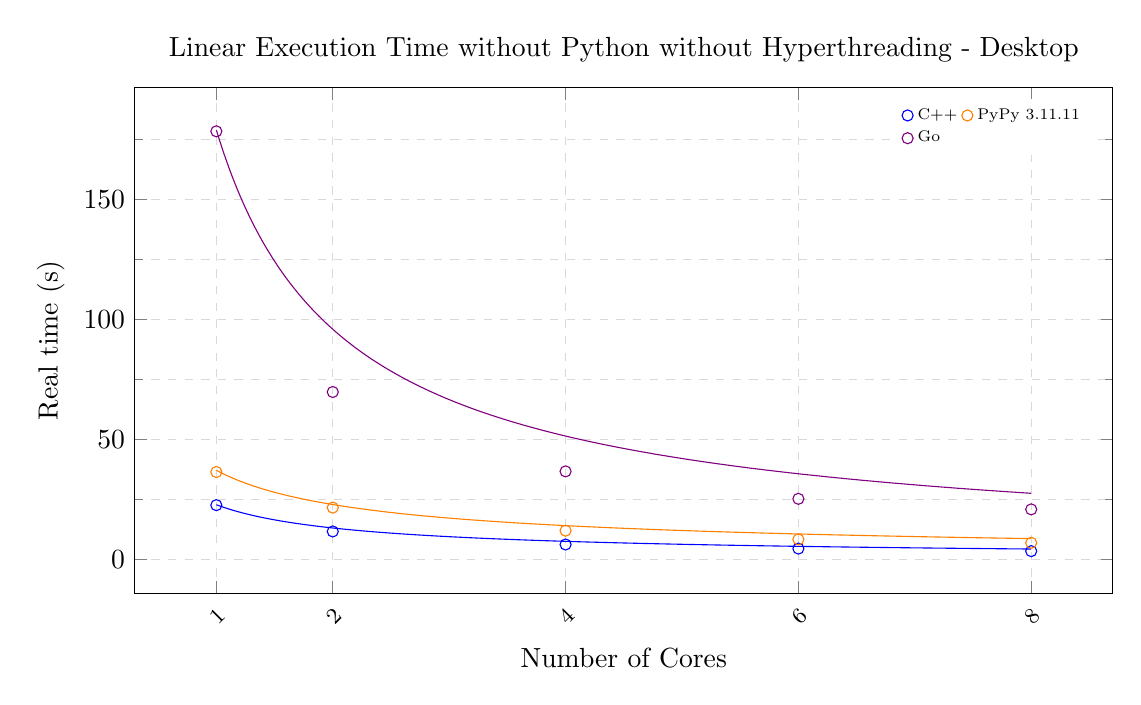
\begin{tikzpicture}
  \begin{axis}[
      title={Linear Execution Time without Python without Hyperthreading - Desktop},
      width=\plotwidthgraph,
      height=\plotheightgraph,
      xlabel={Number of Cores},
      ylabel={Real time (s)},
      ymode=linear,
      xmode=linear,
      grid=both,
      minor tick num=1,
      grid style={gray!30,dashed},
      xtick={1,2,4,6,8},
      x tick label style={
        font=\footnotesize,
        rotate=45,
        anchor=north east
      },
      legend style={
        at={(0.98,0.98)},
        anchor=north east,
        font=\scriptsize,
        nodes={scale=0.8,transform shape},
        draw=none
      },
      legend columns=2,
      transpose legend,
      legend cell align=left,
    ]
    %% C++ %%
    \addplot[
      blue,
      only marks,
      mark=o,
      mark options={draw=blue,fill=white}
    ]
    table[row sep=\\] {
      x   y     \\
      1   22.60 \\
      2   11.64 \\
      4   6.20  \\
      6   4.49  \\
      8   3.43  \\
    };
    \addlegendentry{C++}
    % power-law fit: y = 22.60 * x^(-0.8)
    \addplot[
      blue,
      forget plot,
      domain=1:8,
      samples=200
    ] {22.78 * x^(-0.8)};

    %% Go %%
    \addplot[
      violet,
      only marks,
      mark=o,
      mark options={draw=violet,fill=white}
    ]
    table[row sep=\\] {
      x   y      \\
      1   178.43 \\
      2   69.77  \\
      4   36.68  \\
      6   25.24  \\
      8   20.84  \\
    };
    \addlegendentry{Go}
    % power-law fit: y = 178.43 * x^(-0.9)
    \addplot[
      violet,
      forget plot,
      domain=1:8,
      samples=200
    ] {178.98 * x^(-0.9)};

    %% PyPy 3.11.11 %%
    \addplot[
      orange,
      only marks,
      mark=o,
      mark options={draw=orange,fill=white}
    ]
    table[row sep=\\] {
      x   y      \\
      1   36.42  \\
      2   21.59  \\
      4   11.97  \\
      6   8.35   \\
      8   6.91   \\
    };
    \addlegendentry{PyPy 3.11.11}
    % power-law fit: y = 36.42 * x^(-0.7)
    \addplot[
      orange,
      forget plot,
      domain=1:8,
      samples=200
    ] {37.12 * x^(-0.7)};

  \end{axis}
\end{tikzpicture}
    \caption{Desktop - Linear execution Time without Hyperthreading}{Linear execution time of the laptop benchmark without Hyperthreading across different programming languages without Python.}
    \label{fig:linear-desktop-execution-time-no-hyperthreading}
\end{figure}


\begin{figure}
    \centering
    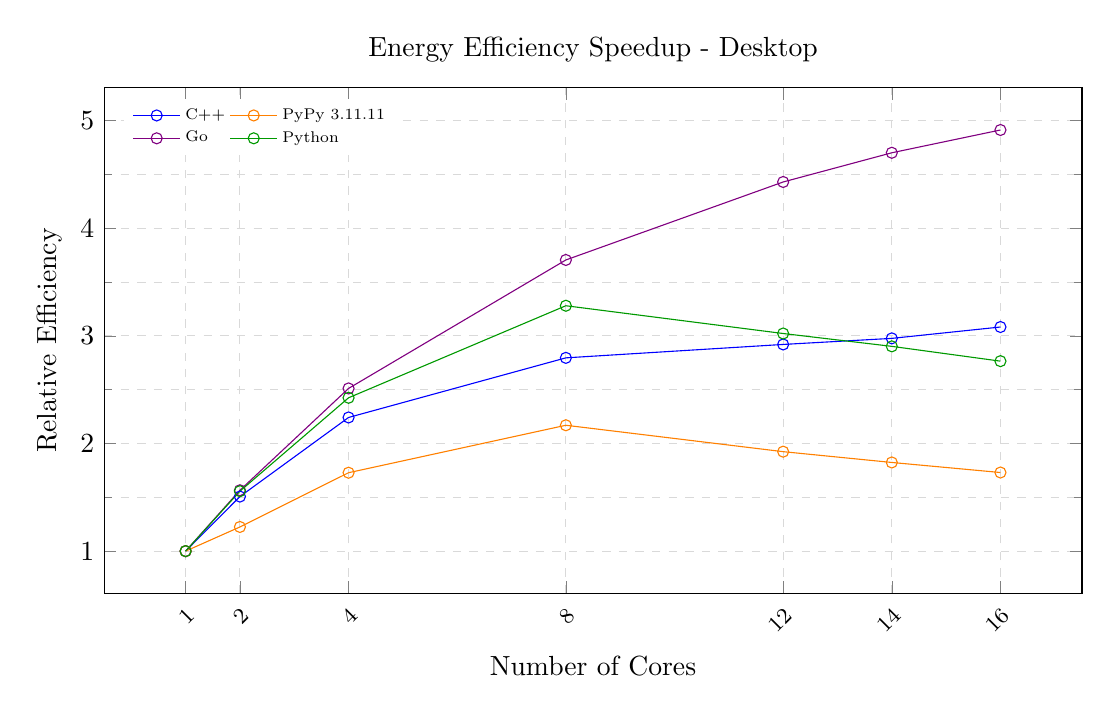
\begin{tikzpicture}
  \begin{axis}[
      title={Energy Efficiency Speedup - Desktop},
      width=\plotwidthgraph,
      height=\plotheightgraph,
      xlabel={Number of Cores},
      ylabel={Relative Efficiency},
      ymode=linear,
      xmode=linear,
      grid=both,
      minor tick num=1,
      grid style={gray!30,dashed},
      xtick={1,2,4,8,12,14,16},
      x tick label style={
        font=\footnotesize,
        rotate=45,
        anchor=north east
      },
      legend style={
        at={(0.02,0.98)},
        anchor=north west,
        font=\scriptsize,
        nodes={scale=0.8,transform shape},
        draw=none
      },
      legend columns=2,
      transpose legend,
      legend cell align=left,
    ]
    %% C++ %%
    \addplot[
      blue,
      mark=o,
    ]
    table[row sep=\\] {
      x   y     \\
      1   1 \\
      2   1.507304763 \\
      4   2.242327612 \\
      8   2.796316665 \\
      12  2.920958049 \\
      14  2.977358037 \\
      16  3.082991294 \\
    };
    \addlegendentry{C++}

    %% Go %%
    \addplot[
      violet,
      mark=o,
    ]
    table[row sep=\\] {
      x   y     \\
      1   1 \\
      2   1.565922217 \\
      4   2.51216421 \\
      8   3.7060202 \\
      12  4.430729033 \\
      14  4.702083667 \\
      16  4.913829636 \\
    };
    \addlegendentry{Go}

    %% PyPy 3.11.11 %%
    \addplot[
      orange,
      mark=o,
    ]
    table[row sep=\\] {
      x   y     \\
      1   1 \\
      2   1.224855557 \\
      4   1.728929021 \\
      8   2.169853226 \\
      12  1.924538378 \\
      14  1.824201658 \\
      16  1.730774156 \\
    };
    \addlegendentry{PyPy 3.11.11}

    %% Python %%
    \addplot[
      green!60!black,
      mark=o,
    ]
    table[row sep=\\] {
      x   y     \\
      1   1 \\
      2   1.557213926 \\
      4   2.425306233 \\
      8   3.280598124 \\
      12  3.022507745 \\
      14  2.903193084 \\
      16  2.765595611 \\
    };
    \addlegendentry{Python}

  \end{axis}
\end{tikzpicture}
    \caption{Desktop - Energy Efficiency Speedup}{Energy efficiency speedup of the Desktop benchmark across different programming languages.}
    \label{fig:desktop-speedup}
\end{figure}


These results show a clear trend in the energy consumption and execution time of the different programming languages. The C++ implementation is the most energy-efficient, as expected, but again, PyPy surprises with its results, being the second most energy-efficient and being much closer to the \gls{CPP} implementation than the Go implementation, which is the third most energy-efficient. Specific numbers for energy consumption and execution time can be found in \autoref{tab:desktop-energy-pkg-hyperthreading} and \autoref{tab:desktop-execution-time-hyperthreading}.

We can also observe from \autoref{fig:linear-desktop-energy-hyperthreading} and \autoref{fig:linear-desktop-execution-time-hyperthreading} that the difference between the 8-core and 16-core tests is less pronounced compared to the server. This is because the processor has only 8 physical cores, while the remaining 8 are hyperthreaded cores, which are less powerful than the physical ones. 

This can also be seen very clearly in the energy consumption of the PyPy and Python tests in \autoref{fig:linear-desktop-energy-hyperthreading} (\autoref{tab:desktop-energy-pkg-hyperthreading}) that when using more than 8 cores makes the energy consumption as the number of threads use separates from 8 (the number of real cores). This also affects the execution time but not as significantly, as we can see in \autoref{fig:linear-desktop-execution-time-hyperthreading} (\autoref{tab:desktop-execution-time-hyperthreading}), where the execution time does not change much when using more than 8 cores, but the energy consumption does.

All the raw data for the benchmarks can be found in the \autoref{chap:appendix-desktop-benchmarks}.

\subsection{Laptop}
This laptop is said to have one of the fastest single-core performance in the market. It has a 14 core \gls{ARM} processor, using the big.LITTLE architecture, with 10 high performance cores and 4 high efficiency cores. It has 48GB of RAM, which is enough to run any of the tests.


This platform is a personal laptop, with a 14 core processor, the Apple M4 Pro, which has 10 high performance cores and 4 high efficiency cores, which is a big.LITTLE architecture. This means that the high performance cores are used for CPU intensive tasks, while the high efficiency cores are used for less demanding tasks, such as web browsing or watching videos. But as Apple does not allow the user setting the cores to be used by a specific process, like it happens on Linux, we can not test the high efficiency cores isolated from the high performance cores, as the operating system will decide for us which cores to use for each process. 

\subsubsection{Cache \& Numa}

\begin{lstlisting}[language=bash, caption={Cache of the Apple M4 Pro by performance level}, label={lst:apple-cache}]
Performance Level 0 (High-Performance Cores (10x)):
  Level   Type   Size
  L1d     Data   128 KB
  L1i     Inst   192 KB
  L2      Uni    16 MB

Performance Level 1 (Efficiency Cores (4x)):
  Level   Type   Size
  L1d     Data   64 KB
  L1i     Inst   128 KB
  L2      Uni    4 MB
\end{lstlisting}

\subsubsection{Results}

\begin{figure}
    \centering
    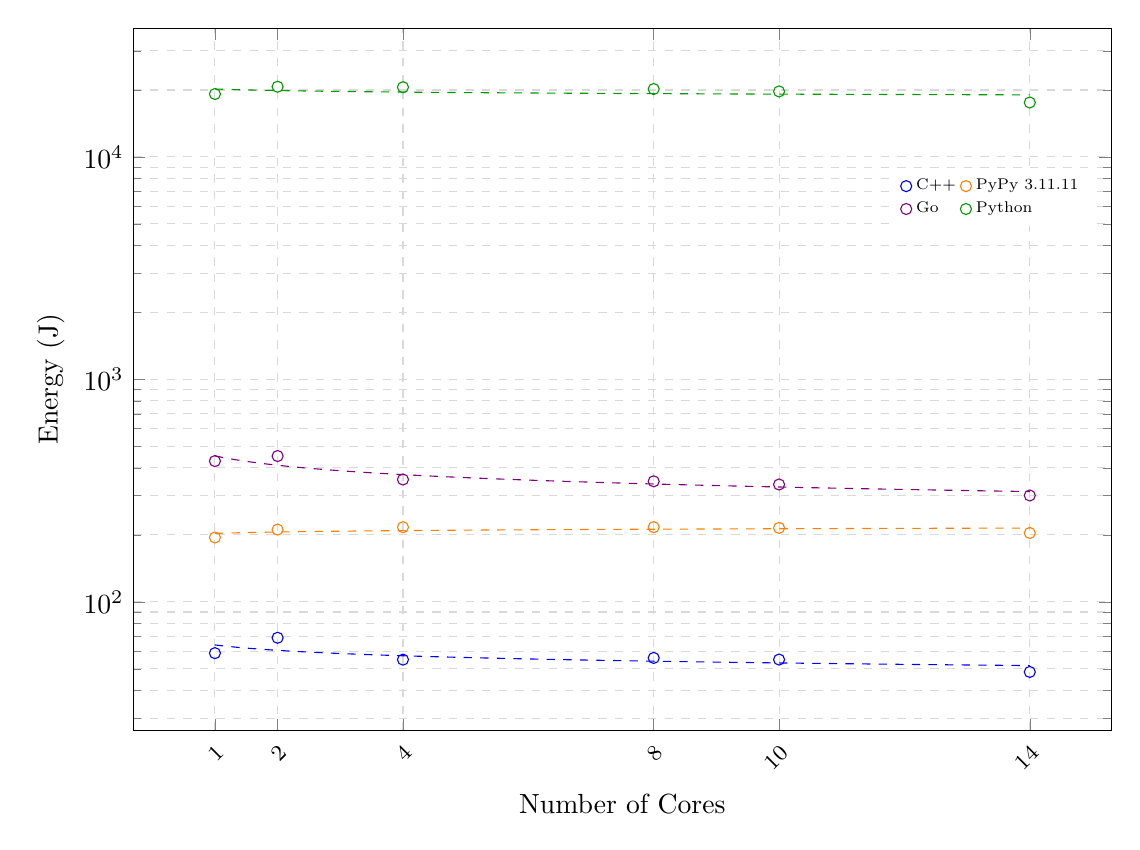
\begin{tikzpicture}
    %% Add a title for the figure
  \begin{semilogyaxis}[
      width=14cm,
      height=10.5cm,
      xlabel={Number of Cores},
      ylabel={Energy (J)},
      ymode=log,
      xmode=linear,
      grid=both,
      minor tick num=1,
      grid style={gray!30,dashed},
      xtick={1,2,4,8,10,14},
      x tick label style={
        font=\footnotesize,
        rotate=45,
        anchor=north east
      },
      legend style={
        at={(0.98,0.8)},
        anchor=north east,
        font=\scriptsize,
        nodes={scale=0.8,transform shape},
        draw=none
      },
      legend columns=2,
      transpose legend,
      legend cell align=left,
    ]
    %% C++ %%
    \addplot[
      blue,
      only marks,
      mark=o,
      mark options={draw=blue,fill=white}
    ]
    table[row sep=\\] {
      x    y      \\
      1    58.79  \\
      2    68.93  \\
      4    54.97  \\
      8    55.94  \\
      10   55.00  \\
      14   48.39  \\
    };
    \addlegendentry{C++}
    % power‐law fit: y = 64.0 * x^(–0.081)
    \addplot[
      blue,
      dashed,
      forget plot,
      domain=1:14,
      samples=200
    ] {64.0 * x^(-0.081)};

    %% Go %%
    \addplot[
      violet,
      only marks,
      mark=o,
      mark options={draw=violet,fill=white}
    ]
    table[row sep=\\] {
      x     y       \\
      1     429.23  \\
      2     452.12  \\
      4     354.64  \\
      8     348.14  \\
      10    336.88  \\
      14    300.66  \\
    };
    \addlegendentry{Go}
    % power‐law fit: y = 453 * x^(–0.140)
    \addplot[
      violet,
      dashed,
      forget plot,
      domain=1:14,
      samples=200
    ] {453 * x^(-0.140)};

    %% PyPy 3.11.11 %%
    \addplot[
      orange,
      only marks,
      mark=o,
      mark options={draw=orange,fill=white}
    ]
    table[row sep=\\] {
      x    y      \\
      1    194.69 \\
      2    211.21 \\
      4    216.53 \\
      8    216.60 \\
      10   214.96 \\
      14   203.92 \\
    };
    \addlegendentry{PyPy 3.11.11}
    % power‐law fit: y = 203 * x^(0.021)
    \addplot[
      orange,
      dashed,
      forget plot,
      domain=1:14,
      samples=200
    ] {203 * x^(0.021)};

    %% Python %%
    \addplot[
      green!60!black,
      only marks,
      mark=o,
      mark options={draw=green!60!black,fill=white}
    ]
    table[row sep=\\] {
      x      y        \\
      1      19183.95 \\
      2      20680.94 \\
      4      20580.73 \\
      8      20198.35 \\
      10     19701.50 \\
      14     17567.03 \\
    };
    \addlegendentry{Python}
    % power‐law fit: y = 20200 * x^(–0.023)
    \addplot[
      green!60!black,
      dashed,
      forget plot,
      domain=1:14,
      samples=200
    ] {20200 * x^(-0.023)};

  \end{semilogyaxis}
\end{tikzpicture}
    \caption{Logarithm Energy consumption of the MBP algorithm in different programming languages.}
    \label{fig:log-mbp-energy}
\end{figure}

\begin{figure}
    \centering
    
    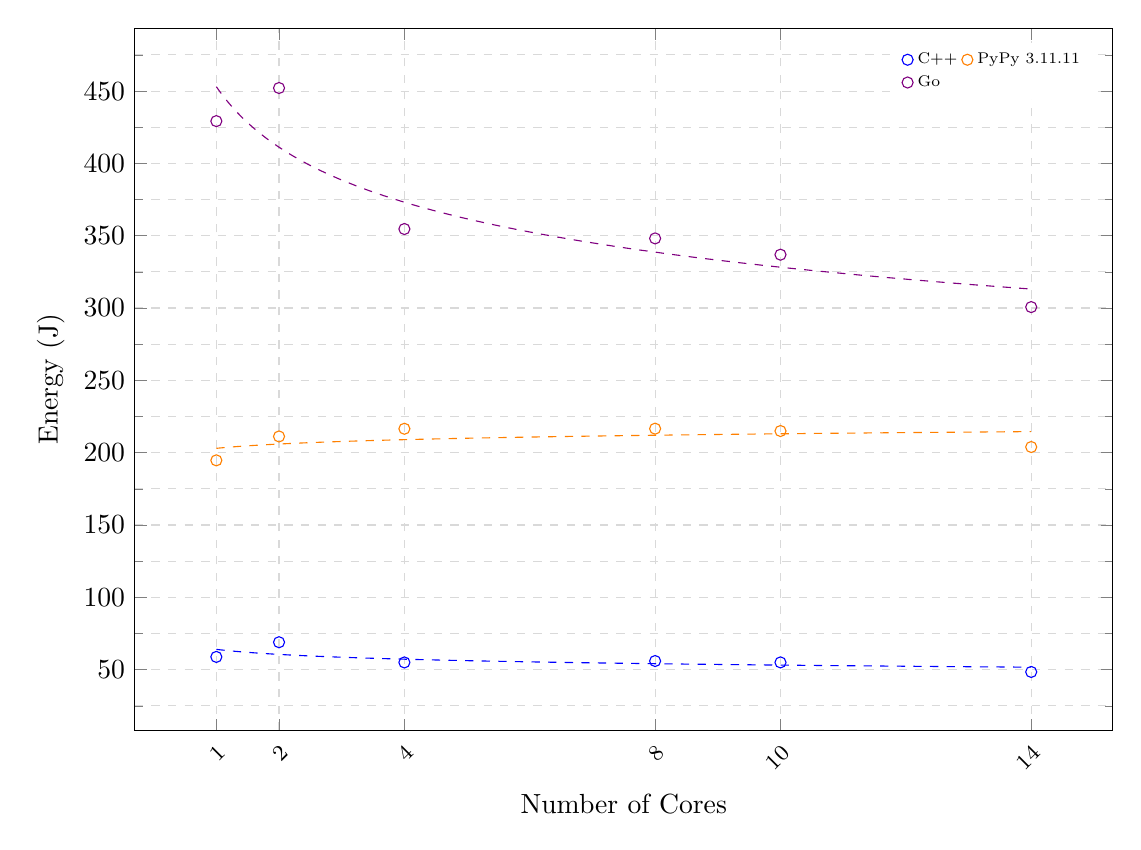
\begin{tikzpicture}
  \begin{axis}[
      width=14cm,
      height=10.5cm,
      xlabel={Number of Cores},
      ylabel={Energy (J)},
      ymode=linear,
      xmode=linear,
      grid=both,
      minor tick num=1,
      grid style={gray!30,dashed},
      xtick={1,2,4,8,10,14},
      x tick label style={
        font=\footnotesize,
        rotate=45,
        anchor=north east
      },
      legend style={
        at={(0.98,0.98)},
        anchor=north east,
        font=\scriptsize,
        nodes={scale=0.8,transform shape},
        draw=none
      },
      legend columns=2,
      transpose legend,
      legend cell align=left,
    ]
    %% C++ %%
    \addplot[
      blue,
      only marks,
      mark=o,
      mark options={draw=blue,fill=white}
    ]
    table[row sep=\\] {
      x    y      \\
      1    58.79  \\
      2    68.93  \\
      4    54.97  \\
      8    55.94  \\
      10   55.00  \\
      14   48.39  \\
    };
    \addlegendentry{C++}
    % power‐law fit: y = 64.0 * x^(–0.081)
    \addplot[
      blue,
      dashed,
      forget plot,
      domain=1:14,
      samples=200
    ] {64.0 * x^(-0.081)};

    %% Go %%
    \addplot[
      violet,
      only marks,
      mark=o,
      mark options={draw=violet,fill=white}
    ]
    table[row sep=\\] {
      x     y       \\
      1     429.23  \\
      2     452.12  \\
      4     354.64  \\
      8     348.14  \\
      10    336.88  \\
      14    300.66  \\
    };
    \addlegendentry{Go}
    % power‐law fit: y = 453 * x^(–0.140)
    \addplot[
      violet,
      dashed,
      forget plot,
      domain=1:14,
      samples=200
    ] {453 * x^(-0.140)};

    %% PyPy 3.11.11 %%
    \addplot[
      orange,
      only marks,
      mark=o,
      mark options={draw=orange,fill=white}
    ]
    table[row sep=\\] {
      x    y      \\
      1    194.69 \\
      2    211.21 \\
      4    216.53 \\
      8    216.60 \\
      10   214.96 \\
      14   203.92 \\
    };
    \addlegendentry{PyPy 3.11.11}
    % power‐law fit: y = 203 * x^(0.021)
    \addplot[
      orange,
      dashed,
      forget plot,
      domain=1:14,
      samples=200
    ] {203 * x^(0.021)};

  \end{axis}
\end{tikzpicture}

    \caption{Linear Energy consumption of the MBP algorithm in different programming languages.}
    \label{fig:linear-mbp-energy}
\end{figure}

\begin{table}
    \centering
    \begin{tabular}{lrrrr}
        \hline
        Cores & C++   & Go     & PyPy 3.11.11 & Python      \\
        \hline
        1     & 58.79  & 429.23  & 194.69       & 19,183.95   \\
        2     & 68.93  & 452.12  & 211.21       & 20,680.94   \\
        4     & 54.97  & 354.64  & 216.53       & 20,580.73   \\
        8     & 55.94  & 348.14  & 216.60       & 20,198.35   \\
        10    & 55.00  & 336.88  & 214.96       & 19,701.50   \\
        14    & 48.39  & 300.66  & 203.92       & 17,567.03   \\
        \hline
    \end{tabular}
    \caption{Power consumption by implementation and core count}
    \label{tab:mbp-power-consumption}
\end{table}

\begin{figure}
    \centering
    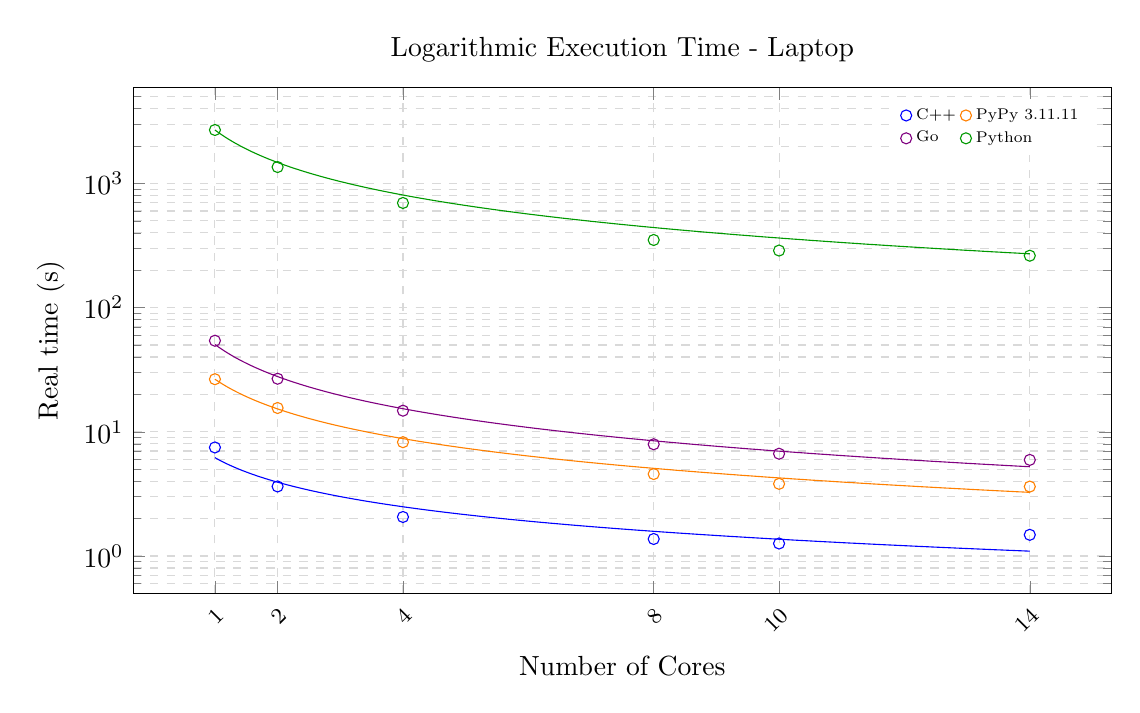
\begin{tikzpicture}
  \begin{semilogyaxis}[
      title={Logarithmic Execution Time - Laptop},
      width=\plotwidthgraph,
      height=\plotheightgraph,
      xlabel={Number of Cores},
      ylabel={Real time (s)},
      ymode=log,
      xmode=linear,
      grid=both,
      minor tick num=1,
      grid style={gray!30,dashed},
      xtick={1,2,4,8,10,14},
      x tick label style={
        font=\footnotesize,
        rotate=45,
        anchor=north east
      },
      legend style={
        at={(0.98,0.98)},
        anchor=north east,
        font=\scriptsize,
        nodes={scale=0.8,transform shape},
        draw=none
      },
      legend columns=2,
      transpose legend,
      legend cell align=left,
    ]
    %% C++ %%
    \addplot[
      blue,
      only marks,
      mark=o,
      mark options={draw=blue,fill=white}
    ]
    table[row sep=\\] {
      x   y     \\
      1   7.48  \\
      2   3.63  \\
      4   2.06  \\
      8   1.37  \\
      10  1.26  \\
      14  1.48  \\
    };
    \addlegendentry{C++}
    % power‐law fit: y = 6.19 * x^(–0.657)
    \addplot[
      blue,
      forget plot,
      domain=1:14,
      samples=200
    ] {6.19 * x^(-0.657)};

    %% Go %%
    \addplot[
      violet,
      only marks,
      mark=o,
      mark options={draw=violet,fill=white}
    ]
    table[row sep=\\] {
      x   y      \\
      1   54.16  \\
      2   26.76  \\
      4   14.80  \\
      8   7.94   \\
      10  6.66   \\
      14  5.94   \\
    };
    \addlegendentry{Go}
    % power‐law fit: y = 50.5 * x^(–0.859)
    \addplot[
      violet,
      forget plot,
      domain=1:14,
      samples=200
    ] {50.5 * x^(-0.859)};

    %% PyPy 3.11.11 %%
    \addplot[
      orange,
      only marks,
      mark=o,
      mark options={draw=orange,fill=white}
    ]
    table[row sep=\\] {
      x   y      \\
      1   26.52  \\
      2   15.55  \\
      4   8.25   \\
      8   4.57   \\
      10  3.81   \\
      14  3.62   \\
    };
    \addlegendentry{PyPy 3.11.11}
    % power‐law fit: y = 26.52 * x^(–0.795)
    \addplot[
      orange,
      forget plot,
      domain=1:14,
      samples=200
    ] {26.52 * x^(-0.795)};

    %% Python %%
    \addplot[
      green!60!black,
      only marks,
      mark=o,
      mark options={draw=green!60!black,fill=white}
    ]
    table[row sep=\\] {
      x    y       \\
      1    2697.08 \\
      2    1356.76 \\
      4    696.75  \\
      8    350.76  \\
      10   288.37  \\
      14   262.00  \\
    };
    \addlegendentry{Python}
    % power‐law fit: y = 2697 * x^(–0.870)
    \addplot[
      green!60!black,
      forget plot,
      domain=1:14,
      samples=200
    ] {2697 * x^(-0.870)};

  \end{semilogyaxis}
\end{tikzpicture}
    \caption{Laptop - Logarithmic Execution Time}{Logarithm Execution time of the Laptop benchmark across different programming languages.}
    \label{fig:log-mbp-execution-time}
\end{figure}

\begin{figure}
    \centering
    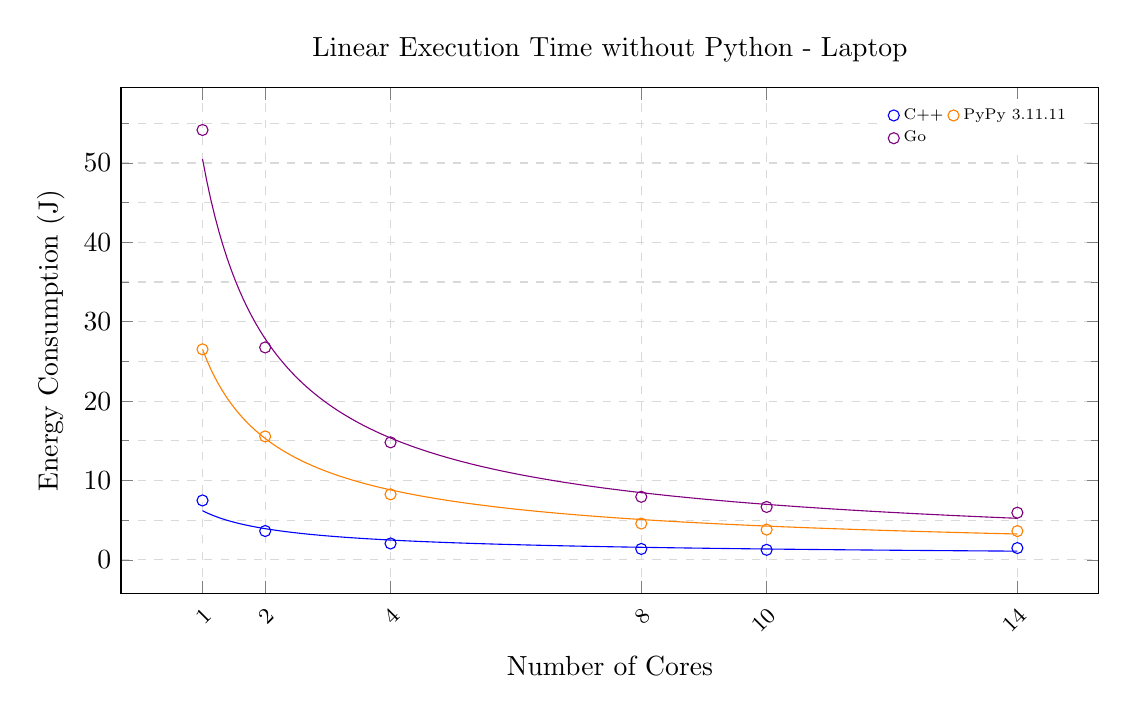
\begin{tikzpicture}
  \begin{axis}[
      title={Linear Execution Time without Python - Laptop},
      width=\plotwidthgraph,
      height=\plotheightgraph,
      xlabel={Number of Cores},
      ylabel={Energy Consumption (J)},
      ymode=linear,
      xmode=linear,
      grid=both,
      minor tick num=1,
      grid style={gray!30,dashed},
      xtick={1,2,4,8,10,14},
      x tick label style={
        font=\footnotesize,
        rotate=45,
        anchor=north east
      },
      legend style={
        at={(0.98,0.98)},
        anchor=north east,
        font=\scriptsize,
        nodes={scale=0.8,transform shape},
        draw=none
      },
      legend columns=2,
      transpose legend,
      legend cell align=left,
    ]
    %% C++ %%
    \addplot[
      blue,
      only marks,
      mark=o,
      mark options={draw=blue,fill=white}
    ]
    table[row sep=\\] {
      x   y     \\
      1   7.48  \\
      2   3.63  \\
      4   2.06  \\
      8   1.37  \\
      10  1.26  \\
      14  1.48  \\
    };
    \addlegendentry{C++}
    % power‐law fit: y = 6.19 * x^(–0.657)
    \addplot[
      blue,
      forget plot,
      domain=1:14,
      samples=200
    ] {6.19 * x^(-0.657)};

    %% Go %%
    \addplot[
      violet,
      only marks,
      mark=o,
      mark options={draw=violet,fill=white}
    ]
    table[row sep=\\] {
      x   y      \\
      1   54.16  \\
      2   26.76  \\
      4   14.80  \\
      8   7.94   \\
      10  6.66   \\
      14  5.94   \\
    };
    \addlegendentry{Go}
    % power‐law fit: y = 50.5 * x^(–0.859)
    \addplot[
      violet,
      forget plot,
      domain=1:14,
      samples=200
    ] {50.5 * x^(-0.859)};

    %% PyPy 3.11.11 %%
    \addplot[
      orange,
      only marks,
      mark=o,
      mark options={draw=orange,fill=white}
    ]
    table[row sep=\\] {
      x   y      \\
      1   26.52  \\
      2   15.55  \\
      4   8.25   \\
      8   4.57   \\
      10  3.81   \\
      14  3.62   \\
    };
    \addlegendentry{PyPy 3.11.11}
    % power‐law fit: y = 26.52 * x^(–0.795)
    \addplot[
      orange,
      forget plot,
      domain=1:14,
      samples=200
    ] {26.52 * x^(-0.795)};

  \end{axis}
\end{tikzpicture}
    \caption{Laptop - Linear execution Time}{Linear execution time of the laptop benchmark across different programming languages without Python.}
    \label{fig:linear-mbp-execution-time}
\end{figure}


\begin{figure}
    \centering
    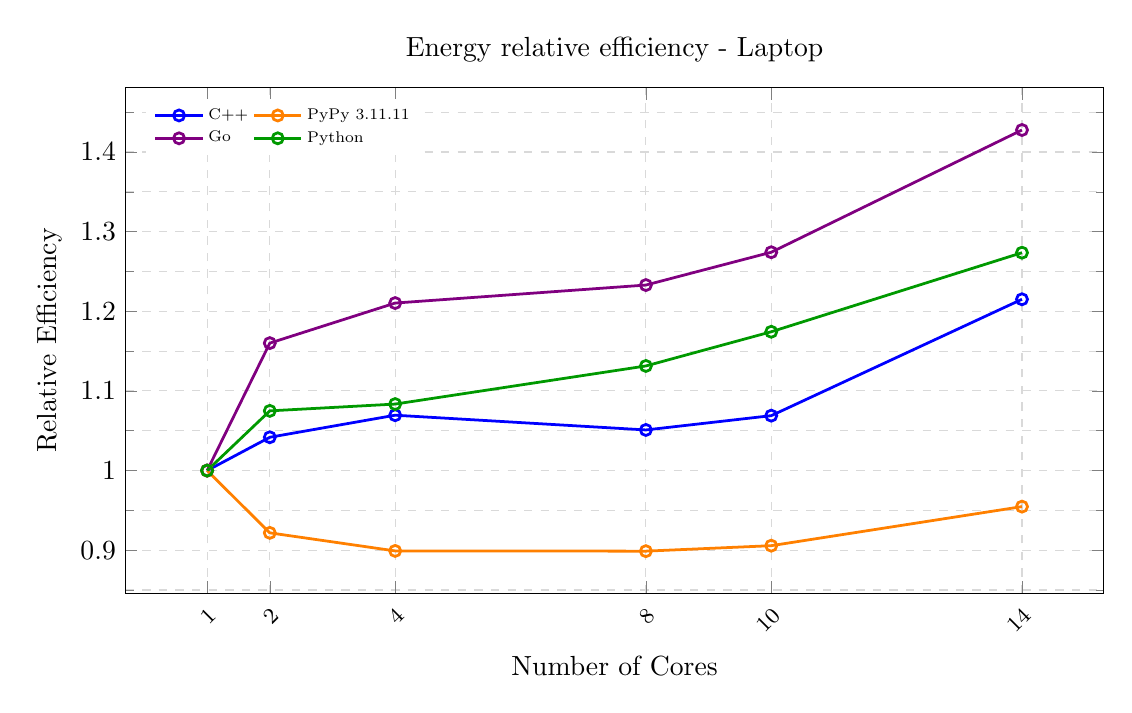
\begin{tikzpicture}
  \begin{axis}[
      title={Energy relative efficiency - Laptop},
      width=\plotwidthgraph,
      height=\plotheightgraph,
      xlabel={Number of Cores},
      ylabel={Relative Efficiency},
      ymode=linear,
      xmode=linear,
      grid=both,
      minor tick num=1,
      grid style={gray!30,dashed},
      xtick={1,2,4,8,10,14},
      x tick label style={
        font=\footnotesize,
        rotate=45,
        anchor=north east
      },
      legend style={
        at={(0.02,0.98)},
        anchor=north west,
        font=\scriptsize,
        nodes={scale=0.8,transform shape},
        draw=none
      },
      legend columns=2,
      transpose legend,
      legend cell align=left,
    ]
    %% C++ %%
    \addplot[
      blue,
      mark=o,
      line width=1pt,
    ]
    table[row sep=\\] {
      x   y     \\
      1   1 \\
      2   1.041812436 \\
      4   1.069494819 \\
      8   1.050991109 \\
      10  1.06893843 \\
      14  1.215060831 \\
    };
    \addlegendentry{C++}

    %% Go %%
    \addplot[
      violet,
      mark=o,
      line width=1pt,
    ]
    table[row sep=\\] {
      x   y     \\
      1   1 \\
      2   1.160033617 \\
      4   1.210314987 \\
      8   1.232920914 \\
      10  1.274120302 \\
      14  1.427607056 \\
    };
    \addlegendentry{Go}

    %% PyPy 3.11.11 %%
    \addplot[
      orange,
      mark=o,
      line width=1pt,
    ]
    table[row sep=\\] {
      x   y     \\
      1   1 \\
      2   0.9217920879 \\
      4   0.8991166162 \\
      8   0.8988151816 \\
      10  0.9056839419 \\
      14  0.9547354298 \\
    };
    \addlegendentry{PyPy 3.11.11}

    %% Python %%
    \addplot[
      green!60!black,
      mark=o,
      line width=1pt,
    ]
    table[row sep=\\] {
      x   y     \\
      1   1 \\
      2   1.074956681 \\
      4   1.083492072 \\
      8   1.131338076 \\
      10  1.174270223 \\
      14  1.273544411 \\
    };
    \addlegendentry{Python}

  \end{axis}
\end{tikzpicture}
    \caption{Laptop - Energy relative efficiency}{Energy relative efficiency of the Laptop benchmark across different programming languages.}
    \label{fig:laptop-relative-energy}
\end{figure}

\begin{figure}
    \centering
    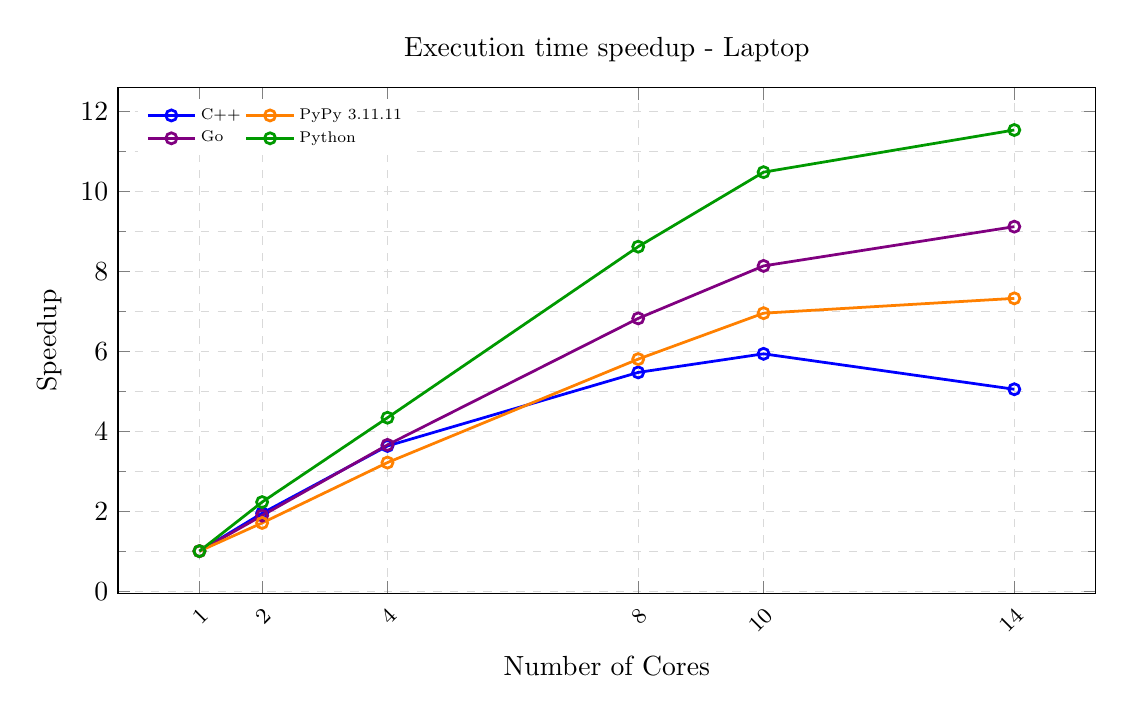
\begin{tikzpicture}
  \begin{axis}[
      title={Execution time speedup - Laptop},
      width=\plotwidthgraph,
      height=\plotheightgraph,
      xlabel={Number of Cores},
      ylabel={Speedup},
      ymode=linear,
      xmode=linear,
      grid=both,
      minor tick num=1,
      grid style={gray!30,dashed},
      xtick={1,2,4,8,10,14},
      x tick label style={
        font=\footnotesize,
        rotate=45,
        anchor=north east
      },
      legend style={
        at={(0.02,0.98)},
        anchor=north west,
        font=\scriptsize,
        nodes={scale=0.8,transform shape},
        draw=none
      },
      legend columns=2,
      transpose legend,
      legend cell align=left,
    ]
    %% C++ %%
    \addplot[
      blue,
      mark=o,
      line width=1pt,
    ]
    table[row sep=\\] {
      x   y     \\
      1   1 \\
      2   1.949152542 \\
      4   3.632167153 \\
      8   5.472181552 \\
      10  5.937251787 \\
      14  5.050675676 \\
    };
    \addlegendentry{C++}

    %% Go %%
    \addplot[
      violet,
      mark=o,
      line width=1pt,
    ]
    table[row sep=\\] {
      x   y     \\
      1   1	 \\
      2   1.8899226	 \\
      4   3.659077089	 \\
      8   6.823484944	 \\
      10  8.13671875	 \\
      14  9.11904361	 \\
    };
    \addlegendentry{Go}

    %% PyPy 3.11.11 %%
    \addplot[
      orange,
      mark=o,
      line width=1pt,
    ]
    table[row sep=\\] {
      x   y     \\
      1   1 \\
      2   1.705439815 \\
      4   3.216468591 \\
      8   5.804990151 \\
      10  6.954116413 \\
      14  7.324772162 \\
    };
    \addlegendentry{PyPy 3.11.11}

    %% Python %%
    \addplot[
      green!60!black,
      mark=o,
      line width=1pt,
    ]
    table[row sep=\\] {
      x   y     \\
      1   1 \\
      2   2.227968773 \\
      4   4.338455223 \\
      8   8.617862305 \\
      10  10.48247378 \\
      14  11.53744275 \\
    };
    \addlegendentry{Python}

  \end{axis}
\end{tikzpicture}
    \caption{Laptop - Execution time speedup}{Execution time speedup of the Laptop benchmark across different programming languages.}
    \label{fig:laptop-time-speedup}
\end{figure}

We can see from \autoref{fig:log-mbp-energy} there does not seem to be a big difference between the execution with one or multiple cores, but this is due to the fact that the table has a logarithmic scale. If we take a look at \autoref{fig:linear-mbp-energy}, we can see that the energy consumption decreases substantially with the Go implementation. But, strangely, both the C++ and PyPy implementation do not seem to reduce the energy consumption with multiple cores. This seems to be due to the fact that the Apple M4 Pro has a big.LITTLE architecture, and the operating system is not able to efficiently use the high performance cores when there are more than $10$ cores available, as it is not able to schedule the tasks efficiently. It could also be that the CPU is drawing its maximum power (around $45-50W$) when running the C++ and PyPy implementations, and thus the energy consumption does not change much with the number of cores as these are quite fast. \footnote{This is one of the points that should be studied forward, more testing with \gls{ARM} chips and a better measurement of the power consumption, with a desktop computer such as the Mac Mini.}



Even though the energy consumption does not decrease, the execution time does, as we can see from \autoref{fig:log-mbp-execution-time}. The C++ implementation is the fastest, followed by the PyPy implementation, then the Go implementation, and finally the Python implementation, which is the slowest by a large margin. I also created this \autoref{fig:linear-mbp-execution-time} to better visualize the execution time of each implementation without Python, as it distorts the results due to its slow performance. Raw data for both energy consumption and execution time can be found in \autoref{tab:mbp-power-consumption} and \autoref{tab:mbp-time-execution} respectively.

All the raw data for the benchmarks can be found in the \autoref{chap:appendix-laptop-benchmarks}.

\subsection{Raspberry Pi 5}
This SBC (Single Board Computer) is one of the most popular in the market, and though is is nota great platform for testing the performance of different programming languages its popularity has made it an interesting option as it has much less power requirements than the other alternatives. It has a 4 core \gls{ARM} processor, 8GB of RAM, which is enough to run any of the tests. 

\subsubsection{Results}

\begin{figure}
  \centering
  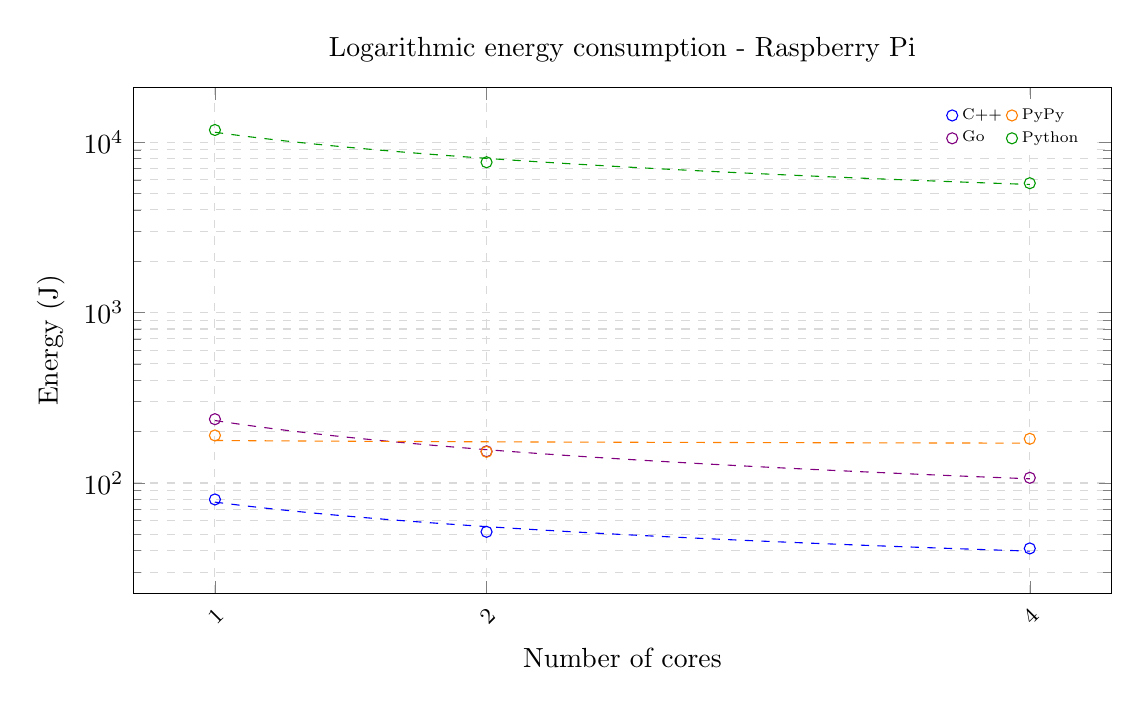
\begin{tikzpicture}
    \begin{semilogyaxis}[
        title={Logarithmic energy consumption - Raspberry Pi},
        width=\plotwidthgraph,
        height=\plotheightgraph,
        xlabel={Number of cores},
        ylabel={Energy (J)},
        ymode=log,
        xmode=linear,
        grid=both,
        minor tick num=1,
        grid style={gray!30,dashed},
        xtick={1,2,4},
        x tick label style={
          font=\footnotesize,
          rotate=45,
          anchor=north east
        },
        legend style={
          at={(0.98,0.98)},
          anchor=north east,
          font=\scriptsize,
          nodes={scale=0.8,transform shape},
          draw=none
        },
        legend columns=2,
        transpose legend,
        legend cell align=left,
      ]

      %% C++ %%
      \addplot[
        blue, only marks, mark=o,
        mark options={draw=blue,fill=white}
      ]
      table[row sep=\\] {
        x   y     \\
        1   80.00  \\
        2   51.67  \\
        4   41.28  \\
      };
      \addlegendentry{C++}
      % fit: y = 77.2 * x^{-0.478}
      \addplot[
        blue, dashed, forget plot,
        domain=1:4, samples=200
      ] {77.2 * x^(-0.478)};

      %% Go %%
      \addplot[
        violet, only marks, mark=o,
        mark options={draw=violet,fill=white}
      ]
      table[row sep=\\] {
        x    y       \\
        1    236.67  \\
        2    153.33  \\
        4    107.20  \\
      };
      \addlegendentry{Go}
      % fit: y = 232.4 * x^{-0.568}
      \addplot[
        violet, dashed, forget plot,
        domain=1:4, samples=200
      ] {232.4 * x^(-0.568)};

      %% PyPy %%
      \addplot[
        orange, only marks, mark=o,
        mark options={draw=orange,fill=white}
      ]
      table[row sep=\\] {
        x    y      \\
        1    190.00 \\
        2    152.33 \\
        4    181.60 \\
      };
      \addlegendentry{PyPy}
      % fit: y = 177.5 * x^{-0.026}
      \addplot[
        orange, dashed, forget plot,
        domain=1:4, samples=200
      ] {177.5 * x^(-0.026)};

      %% Python %%
      \addplot[
        green!60!black, only marks, mark=o,
        mark options={draw=green!60!black,fill=white}
      ]
      table[row sep=\\] {
        x      y        \\
        1      11780.00 \\
        2      7620.67  \\
        4      5739.00  \\
      };
      \addlegendentry{Python}
      % fit: y = 11423 * x^{-0.509}
      \addplot[
        green!60!black, dashed, forget plot,
        domain=1:4, samples=200
      ] {11423 * x^(-0.509)};

    \end{semilogyaxis}
  \end{tikzpicture}
\caption{Raspberry Pi - Logarithmic energy consumption}{Logarithm energy consumption of the Raspberry Pi benchmark across different programming languages.}
\label{fig:log-rpi-energy}
\end{figure}



\begin{figure}
    \centering
  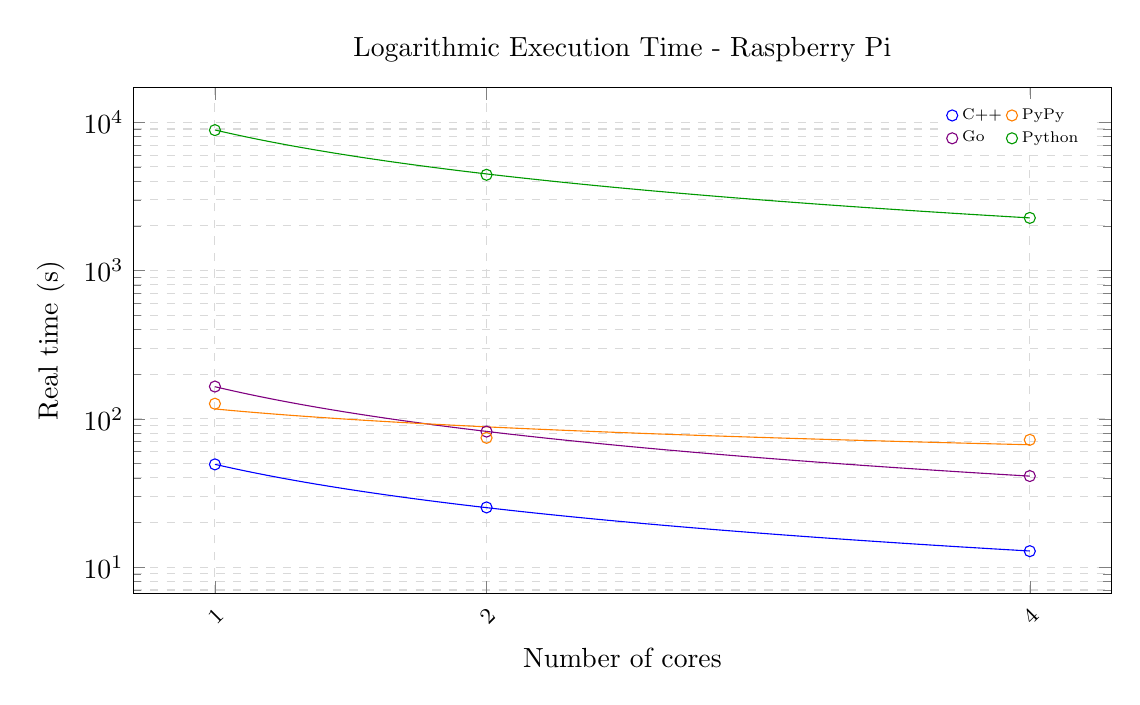
\begin{tikzpicture}
    \begin{semilogyaxis}[
      title={Logarithmic Execution Time - Raspberry Pi},
      width=\plotwidthgraph,
      height=\plotheightgraph,
      xlabel={Number of cores},
      ylabel={Real time (s)},
      ymode=log,
      xmode=linear,
      grid=both,
      minor tick num=1,
      grid style={gray!30,dashed},
      xtick={1,2,4},
      x tick label style={
        font=\footnotesize,
        rotate=45,
        anchor=north east
      },
      legend style={
        at={(0.98,0.98)},
        anchor=north east,
        font=\scriptsize,
        nodes={scale=0.8,transform shape},
        draw=none
      },
      legend columns=2,
      transpose legend,
      legend cell align=left,
    ]

    %% C++ %%
    \addplot[
      blue, only marks, mark=o,
      mark options={draw=blue,fill=white}
    ]
    table[row sep=\\] {
      x   y     \\
      1   49.26  \\
      2   25.25  \\
      4   12.80  \\
    };
    \addlegendentry{C++}
    % fit: y = 49.3 * x^{-0.971}
    \addplot[
      blue, forget plot,
      domain=1:4, samples=200
    ] {49.3 * x^(-0.971)};

    %% Go %%
    \addplot[
      violet, only marks, mark=o,
      mark options={draw=violet,fill=white}
    ]
    table[row sep=\\] {
      x   y      \\
      1   165.03 \\
      2   81.98  \\
      4   41.10  \\
    };
    \addlegendentry{Go}
    % fit: y = 164.6 * x^{-1.002}
    \addplot[
      violet, forget plot,
      domain=1:4, samples=200
    ] {164.6 * x^(-1.002)};

    %% PyPy %%
    \addplot[
      orange, only marks, mark=o,
      mark options={draw=orange,fill=white}
    ]
    table[row sep=\\] {
      x   y      \\
      1   126.36 \\
      2   74.42  \\
      4   72.14  \\
    };
    \addlegendentry{PyPy}
    % fit: y = 116.5 * x^{-0.401}
    \addplot[
      orange, forget plot,
      domain=1:4, samples=200
    ] {116.5 * x^(-0.401)};

    %% Python %%
    \addplot[
      green!60!black, only marks, mark=o,
      mark options={draw=green!60!black,fill=white}
    ]
    table[row sep=\\] {
      x     y       \\
      1     8853.08 \\
      2     4423.91 \\
      4     2264.50 \\
    };
    \addlegendentry{Python}
    % fit: y = 8870 * x^{-0.985}
    \addplot[
      green!60!black, forget plot,
      domain=1:4, samples=200
    ] {8870 * x^(-0.985)};

    \end{semilogyaxis}
  \end{tikzpicture}
\caption{Raspberry Pi - Logarithmic Execution Time}{Logarithm Execution time of the Raspberry Pi benchmark across different programming languages. source: \autoref{tab:rpi-time-execution}}
\label{fig:log-rpi-execution}
\end{figure}


\begin{figure}
    \centering
    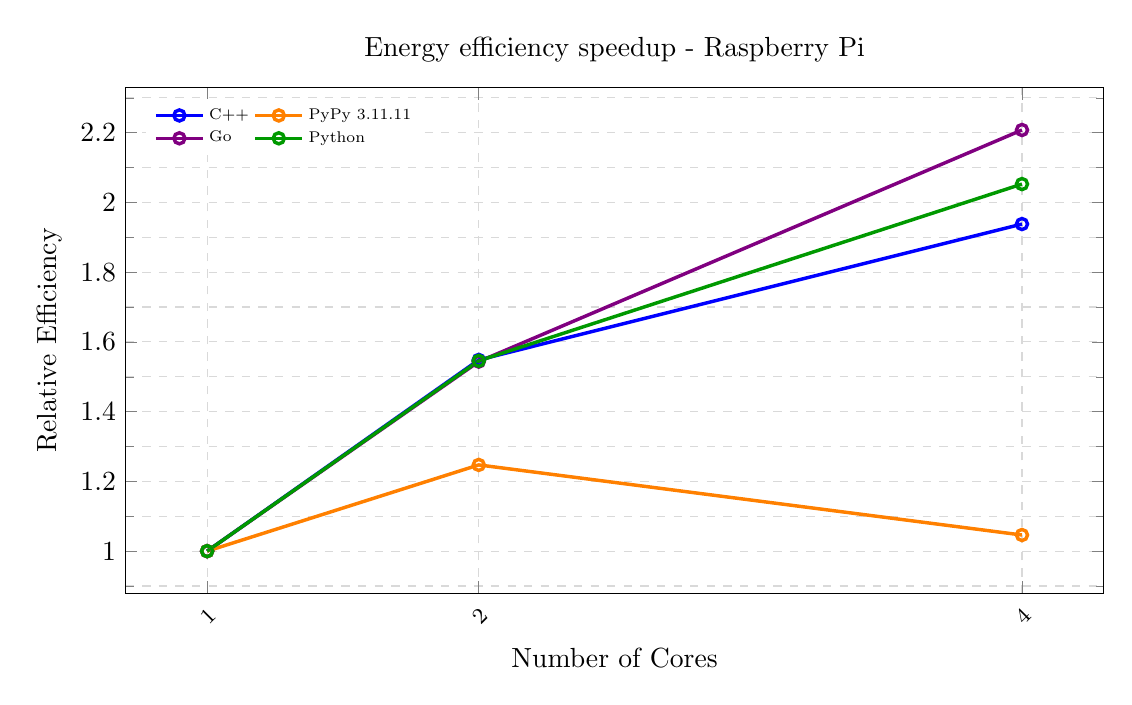
\begin{tikzpicture}
  \begin{axis}[
      title={Energy efficiency speedup - Raspberry Pi},
      width=\plotwidthgraph,
      height=\plotheightgraph,
      xlabel={Number of Cores},
      ylabel={Relative Efficiency},
      ymode=linear,
      xmode=linear,
      grid=both,
      minor tick num=1,
      grid style={gray!30,dashed},
      xtick={1,2,4},
      x tick label style={
        font=\footnotesize,
        rotate=45,
        anchor=north east
      },
      legend style={
        at={(0.02,0.98)},
        anchor=north west,
        font=\scriptsize,
        nodes={scale=0.8,transform shape},
        draw=none
      },
      legend columns=2,
      transpose legend,
      legend cell align=left,
    ]
    %% C++ %%
    \addplot[
      blue,
      mark=o,
      line width=1.25pt,
    ]
    table[row sep=\\] {
      x   y     \\
      1   1 \\
      2   1.548387097 \\
      4   1.937984496 \\
    };
    \addlegendentry{C++}

    %% Go %%
    \addplot[
      violet,
      mark=o,
      line width=1.25pt,
    ]
    table[row sep=\\] {
      x   y     \\
      1   1 \\
      2   1.543478261 \\
      4   2.207711443 \\
    };
    \addlegendentry{Go}

    %% PyPy 3.11.11 %%
    \addplot[
      orange,
      mark=o,
      line width=1.25pt,
    ]
    table[row sep=\\] {
      x   y     \\
      1   1 \\
      2   1.24726477 \\
      4   1.046255507 \\
    };
    \addlegendentry{PyPy 3.11.11}

    %% Python %%
    \addplot[
      green!60!black,
      mark=o,
      line width=1.25pt,
    ]
    table[row sep=\\] {
      x   y     \\
      1   1 \\
      2   1.545796518 \\
      4   2.052622408 \\
    };
    \addlegendentry{Python}

  \end{axis}
\end{tikzpicture}
    \caption{Raspberry Pi - Energy package relative efficiency}{Energy package relative efficiency of the Raspberry Pi benchmark across different programming languages.}
    \label{fig:rpi-relative-energy}
\end{figure}

\begin{figure}
    \centering
    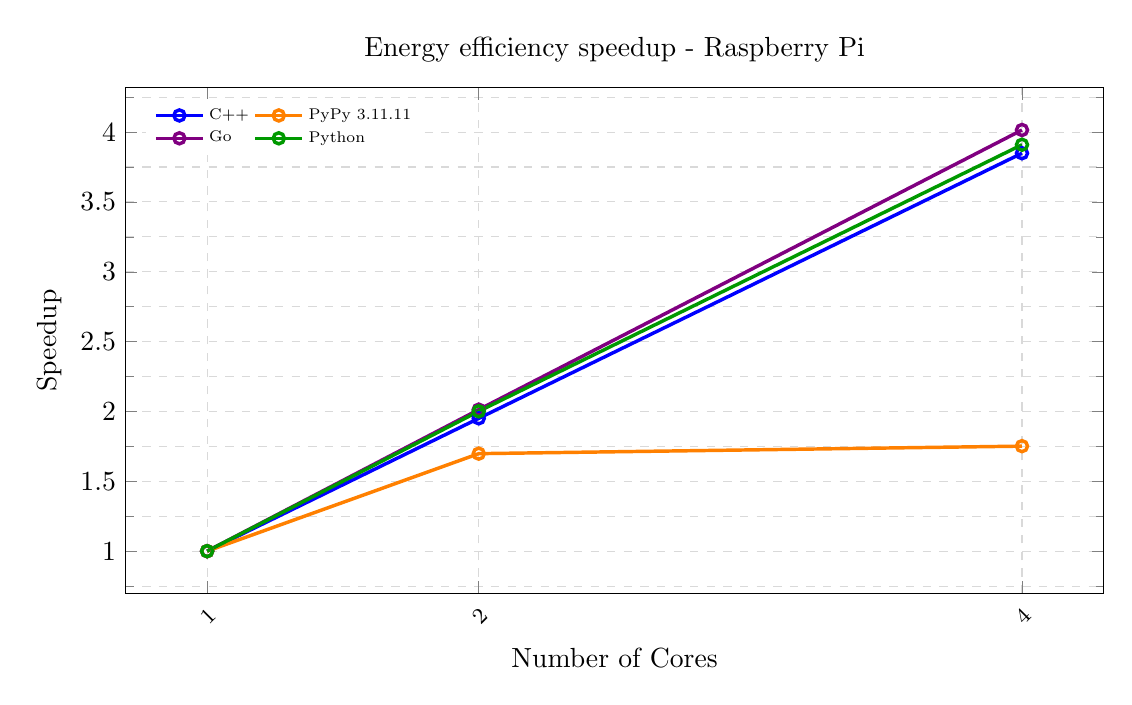
\begin{tikzpicture}
  \begin{axis}[
      title={Energy efficiency speedup - Raspberry Pi},
      width=\plotwidthgraph,
      height=\plotheightgraph,
      xlabel={Number of Cores},
      ylabel={Speedup},
      ymode=linear,
      xmode=linear,
      grid=both,
      minor tick num=1,
      grid style={gray!30,dashed},
      xtick={1,2,4},
      x tick label style={
        font=\footnotesize,
        rotate=45,
        anchor=north east
      },
      legend style={
        at={(0.02,0.98)},
        anchor=north west,
        font=\scriptsize,
        nodes={scale=0.8,transform shape},
        draw=none
      },
      legend columns=2,
      transpose legend,
      legend cell align=left,
    ]
    %% C++ %%
    \addplot[
      blue,
      mark=o,
      line width=1.25pt,
    ]
    table[row sep=\\] {
      x   y     \\
      1   1 \\
      2   1.950877788	 \\
      4   3.848824582	 \\
    };
    \addlegendentry{C++}

    %% Go %%
    \addplot[
      violet,
      mark=o,
      line width=1.25pt,
    ]
    table[row sep=\\] {
      x   y     \\
      1   1 \\
      2   2.013136804 \\
      4   4.015077052 \\
    };
    \addlegendentry{Go}

    %% PyPy 3.11.11 %%
    \addplot[
      orange,
      mark=o,
      line width=1.25pt,
    ]
    table[row sep=\\] {
      x   y     \\
      1   1 \\
      2   1.697986947 \\
      4   1.751732838 \\
    };
    \addlegendentry{PyPy 3.11.11}

    %% Python %%
    \addplot[
      green!60!black,
      mark=o,
      line width=1.25pt,
    ]
    table[row sep=\\] {
      x   y     \\
      1   1 \\
      2   2.001188255 \\
      4   3.909506176 \\
    };
    \addlegendentry{Python}

  \end{axis}
\end{tikzpicture}
    \caption{Raspberry Pi - Execution time speedup}{Energy efficiency speedup of the Raspberry Pi benchmark across different programming languages.}
    \label{fig:rpi-time-speedup}
\end{figure}


From both \autoref{fig:log-rpi-energy} and \autoref{fig:log-rpi-execution} we can see that the trend lines, in this case intersect, meaning that passing from 2 to 4 cores, the energy increases for the PyPy implementation and decreases for the rest of the implementation. This is due to the fact that the Raspberry Pi 5 has a much less powerfull processor and thus, compiled languages such as C++ and Go can obtain better power efficiency results when using more cores, as the processor is able to handle the load better. 

It is impressive the slowness that python shows in this platform, $62$x less power efficient than PyPy and consuming more than $147$x the energy of the C++ implementation. 

If we turn to the execution times, we can see that the C++ implementation is the fastest, followed by the Go implementation, then PyPy and lastly Python when looking at the 4 cores run of the benchmark. But, when the program was run with 2 cores, the PyPy implementation does not reduce much the execution time, compared to the Go result, interchanging the position of the Go and PyPy implementations, as it can be seen in clearer in the raw data in \autoref{chap:appendix-rpi-benchmarks}.

\section{Comment on parallelizing different languages}

In this section, I would like to make some comment on the parallelization on different languages, and why some might experience a different behavior. 

\subsection{Go}
When choosing how many `cores' the tests are using, for the Go implementation, I used the size of the \texttt{waitChan} channel. This number can be changed to be more than the total number of threads in the system, which sometimes increases the performance.

\begin{figure}[htbp]
 \centering
 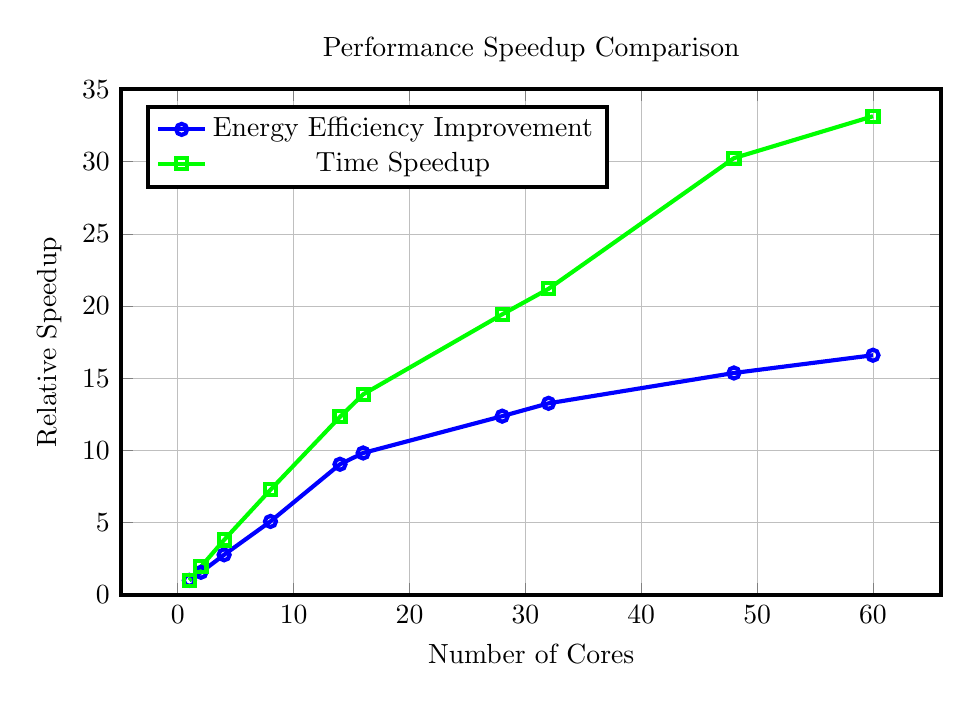
\begin{tikzpicture}
 \begin{axis}[
     xlabel={Number of Cores},
     ylabel={Relative Speedup},
     title={Performance Speedup Comparison},
     grid=both,
     grid style={line width=.1pt, draw=gray!10},
     major grid style={line width=.2pt,draw=gray!50},
     width=12cm,
     height=8cm,
     legend pos=north west,
     mark size=2pt,
     line width=1.5pt,
     ymin=0,
     ymax=35
 ]
 
 % Energy speedup (selected points for clarity)
 \addplot[color=blue, mark=o] coordinates {
     (1, 1)
     (2, 1.56)
     (4, 2.77)
     (8, 5.08)
     (14, 9.04)
     (16, 9.82)
     (28, 12.37)
     (32, 13.26)
     (48, 15.36)
     (60, 16.59)
 };
 
 % Time speedup (selected points for clarity)
 \addplot[color=green, mark=square] coordinates {
     (1, 1)
     (2, 1.94)
     (4, 3.8)
     (8, 7.27)
     (14, 12.32)
     (16, 13.88)
     (28, 19.42)
     (32, 21.19)
     (48, 30.24)
     (60, 33.14)
 };
 
 \legend{Energy Efficiency Improvement, Time Speedup}
\end{axis}
\end{tikzpicture}
\caption{Relative performance improvements showing time scales better than energy efficiency}
\label{fig:go-routines-speedup} 
\end{figure}


\begin{table}
  \centering
  \begin{tabular}{lcrcrc}
    \toprule
    Cores & Goroutines & Energy (J) & Relative Energy & Execution time (s) & Relative Time \\
    \midrule
    1             & 1          &  28,522.69         & ($1x$)              &  172.952          &  ($1x$)               \\
    1             & 2          &  28,919.31         & ($0.99x$)           &  175.381          &  ($0.99x$)            \\
    2             & 2          &  18,231.97         & ($1.56x$)           &   89.319          &  ($1.94x$)            \\
    2             & 4          &  18,224.50         & ($1.57x$)           &   89.275          &  ($1.94x$)            \\
    4             & 4          &  10,304.27         & ($2.77x$)           &   45.508          &  ($3.8x$)             \\
    4             & 8          &  10,299.06         & ($2.77x$)           &   45.482          &  ($3.8x$)             \\
    8             & 8          &  \textbf{5,617.27} & (\textbf{$5.08x$})  &   \textbf{23.781} &  (\textbf{$7.27x$})   \\
    8             & 16         &  5,580.52          & ($5.11x$)           &   23.594          &  ($7.33x$)            \\
    14            & 14         &  3,155.30          & ($9.04x$)           &   14.034          &  ($12.32x$)           \\
    14            & 28         &  3,151.93          & ($9.05x$)           &   14.001          &  ($12.35x$)           \\
    16            & 16         &  2,904.52          & ($9.82x$)           &   12.456          &  ($13.88x$)           \\
    16            & 32         &  3,018.54          & ($9.45x$)           &   12.435          &  ($13.91x$)           \\
    28            & 28         &  2,306.35          & ($12.37x$)          &    8.906          &  ($19.42x$)           \\
    28 \textbf{*} & 28         &  \textbf{2,271.71} & (\textbf{$12.56x$}) &    \textbf{7.613} &  (\textbf{$22.72x$})  \\
    28            & 56         &  2,314.29          & ($12.32x$)          &    7.791          &  ($22.2x$)            \\
    28 \textbf{*} & 56         &  \textbf{2,290.85} & (\textbf{$12.45x$}) &    \textbf{8.815} &  (\textbf{$19.62x$})  \\
    32            & 32         &  2,151.74          & ($13.26x$)          &    8.163          &  ($21.19x$)           \\
    32 \textbf{*} & 32         &  \textbf{2,109.37} & (\textbf{$13.52x$}) &    \textbf{6.822} &  (\textbf{$25.35x$})  \\
    32            & 64         &  2,121.88          & ($13.44x$)          &    8.101          &  ($21.35x$)           \\
    32 \textbf{*} & 64         &  \textbf{2,142.21} & (\textbf{$13.31x$}) &    \textbf{6.896} &  (\textbf{$25.08x$})  \\
    48            & 48         &  1,856.93          & ($15.36x$)          &    5.718          &  ($30.24x$)           \\
    48            & 96         &  1,848.47          & ($15.43x$)          &    5.673          &  ($30.48x$)           \\
    60            & 60         &  1,744.76          & ($16.35x$)          &    5.357          &  ($32.28x$)           \\
    60            & 120        &  1,737.80          & ($16.41x$)          &    5.320          &  ($32.5x$)            \\
    60            & 200        &  1,724.73          & ($16.54x$)          &    5.255          &  ($32.91x$)           \\
    60            & 250        &  1,719.49          & ($16.59x$)          &    5.218          &  ($33.14x$)           \\
    \bottomrule
  \end{tabular}
  \caption[Go goroutines and threads]{Go goroutines and threads used in the tests, where \textbf{*} means the execution has been fixed to a single CPU}
  \label{tab:go-routines-cores}
\end{table}


As it can be seen from \autoref{tab:go-routines-cores}, the Go implementation is able to use more than the total number of threads in the system, and it is able to use them efficiently, as the Go runtime is able to schedule the goroutines efficiently. We can also observe from the table, that the results that are run in the same CPU chip versus different CPU chips, have similar energy consumptions, but the execution times are significantly lower as there are no context switches happening between the two CPUs. This can be seen in the 28 cores same CPU and 32 cores same CPU tests, marked in \autoref{tab:go-routines-cores} with a \textbf{*}.

\subsection{Python}
When iterating though every pixel in Python, as the environment has to be copied for every single pixel, the cores are not being used at 100\% of their capacity, specifically, while testing I saw that the cores were being used at around 5\%-15\% of their capacity. Meaning the creation of too many threads is not beneficial, as the overhead of creating the threads is larger than the actual work being done by each thread. 
Another factor that Python, each time a task is submitted to a process, Python needs to serialize (pickle) the entire world object and other parameters, then deserialize them in the worker process, which means that, if this has to happen for every pixel, the serializing and deserializing tasks run for much longer than the actual pixel processing.

\section{Most efficient language optimizations}
As we can see from these results, the most efficient language in terms of energy consumption and execution time is C++. 

But, out of the box, does C++ always provide the best performance? The answer is no, as the compiler plays an extremely important role in the performance of the code, and the compiler optimizations can make a huge difference in the performance of the code.
For these tests, I tested many optimization flags, such as \texttt{-O3} and \texttt{-march=native}, which allows the compiler to optimize the code for the specific architecture of the machine it is being compiled on. But what would happen if we used different compiler flags, would the results change? Would another language be more efficient?

As to not leave the reader with the intrigue of what would happen if we used different compiler flags, I have compiled and tested all the programs with the following flags:
\begin{itemize}
    \item \texttt{-O0}: No optimizations, the compiler will not optimize the code at all.
    \item \textbf{-O1}: Basic optimizations; the compiler will optimize the code. It performs a basic cleanup, removing dead code and some simple inlining.
    \item \textbf{-O2}: More optimizations; this is the recommended optimization level for most use cases.
    \item \textbf{-O3}: Maximum optimizations, very aggressive optimizations:
    \begin{itemize}
        \item Loop transformations: Unrolling loops even more than \texttt{-O2}, changing the distribution of loops and interchanging them.
        \item Speculative optimizations
        \item Vectorization: \gls{SIMD} instructions (AVX, SSE, etc.)
        \item Predictive commoning (reusing computations from previous loop iterations)
    \end{itemize}
    \item \textbf{-O3 with --fast-math}: Maximum optimizations; the compiler will optimize the code as much as possible, but operations will not be as precise.
\end{itemize}

As \autocite{llvm-fast-math} explains, the \texttt{--fast-math} flag allows the compiler to perform optimizations that may not be mathematically correct, but will result in faster code. 


\begin{table}
  \centering
  \caption{Power/Energy and execution time for various core counts and compiler optimization flags}
  \label{tab:compiler-optimizations}
  \begin{tabular}{lrrrrr}
    \toprule
    \textbf{Metric / Flags} & \textbf{-O0} & \textbf{-O1} & \textbf{-O2} & \textbf{-O3} & \textbf{-O3 (fast-math)} \\
    \midrule
    \multicolumn{6}{c}{\textbf{1 core}} \\
    power/energy-pkg (J) & 52,957.47 & 5,185.28 & 4,388.12 &  4,031.83   & \textbf{4,005.70} \\
    power/energy-ram (J) & 2,208.08  & 210.28   & 183.21   &    180.00   & \textbf{168.52}  \\
    time (s)             & 270.06    & 27.453   & 24.02    &     23.5993 & \textbf{22.054}  \\
    \midrule
    \multicolumn{6}{c}{\textbf{4 cores}} \\
    power/energy-pkg (J) & 13,379.59 & 1,564.51 & 1,417.01 & \textbf{1,386.60} & 1,414.08       \\
    power/energy-ram (J) & 508.40    & 56.72    & 50.96    &     50.37         & \textbf{49.56}  \\
    time (s)             & 66.066    & 7.4351   & 6.67     &    6.5605         & \textbf{6.478}  \\
    \midrule
    \multicolumn{6}{c}{\textbf{14 cores}} \\
    power/energy-pkg (J) & 5,056.15  & 658.46   & 606.58   & \textbf{595.29}  & 639.00         \\
    power/energy-ram (J) & 153.03    & 20.79    & 18.53    & \textbf{18.24}  & 20.10          \\
    time (s)             & 19.9344   & 2.7184   & 2.42     & \textbf{2.3807} & 2.62           \\
    \midrule
    \multicolumn{6}{c}{\textbf{28 cores}} \\
    power/energy-pkg (J) & 3,650.43  & 627.89   & 565.83   &    561.59   & \textbf{547.56} \\
    power/energy-ram (J) & 120.49    & 20.00    & 18.00    &     17.93   & \textbf{17.47}  \\
    time (s)             & 15.729    & 2.6043   & 2.36     &     2.3382  & \textbf{2.2701} \\
    \midrule
    \multicolumn{6}{c}{\textbf{32 cores}} \\
    power/energy-pkg (J) & 3,353.53  & 606.52   & 552.98   &     548.83  & \textbf{535.22} \\
    power/energy-ram (J) & 110.47    & 19.54    & 17.76    &     17.58   & \textbf{17.27}  \\
    time (s)             & 14.4472   & 2.5369   & 2.33     &     2.3015  & \textbf{2.2368} \\
    \midrule
    \multicolumn{6}{c}{\textbf{60 cores}} \\
    power/energy-pkg (J) & 2,794.03  & 698.96   & 661.76   & \textbf{659.31} & 671.51         \\
    power/energy-ram (J) & 86.80     & 25.37    & 24.11    & \textbf{24.10}  & 24.76          \\
    time (s)             & 7.5463    & 1.89955  & 1.80     &     1.79288     & \textbf{1.79288}\\
    \bottomrule
  \end{tabular}
\end{table}

% --- Chart 1: Execution Time ---
\begin{figure}[!ht]
  \centering
  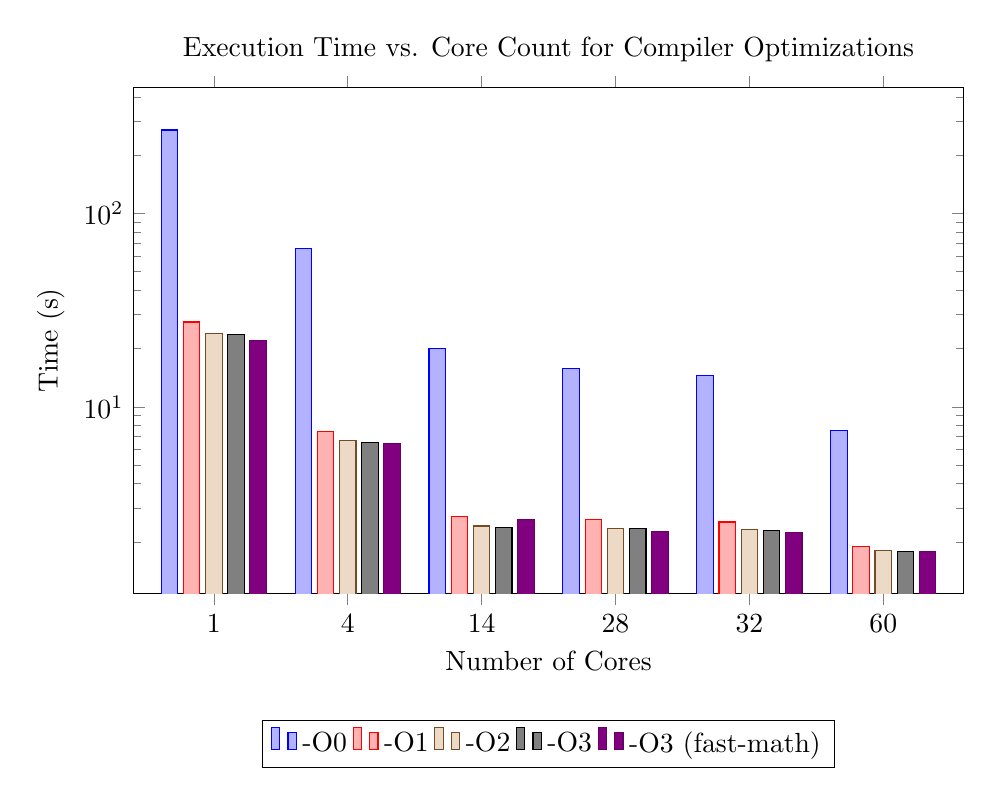
\begin{tikzpicture}
    \begin{axis}[
        title={Execution Time vs. Core Count for Compiler Optimizations},
        width=\textwidth,   
        height=8cm,         
        ybar,               
        ymode=log,          
        log basis y={10},
        enlarge x limits=0.12, 
        xlabel={Number of Cores},
        ylabel={Time (s)},
        symbolic x coords={1, 4, 14, 28, 32, 60},
        xtick=data, 
        bar width=6pt, 
        legend style={
          at={(0.5,-0.25)},
          anchor=north,
          legend columns=-1 
        },
        yticklabel style={
            /pgf/number format/fixed,
            /pgf/number format/precision=2
        },
    ]
    % Add a plot for each optimization flag. pgfplots groups them automatically.
    \addplot coordinates {(1, 270.06) (4, 66.066) (14, 19.9344) (28, 15.729) (32, 14.4472) (60, 7.5463)};
    \addplot coordinates {(1, 27.453) (4, 7.4351) (14, 2.7184) (28, 2.6043) (32, 2.5369) (60, 1.89955)};
    \addplot coordinates {(1, 24.02) (4, 6.67) (14, 2.42) (28, 2.36) (32, 2.33) (60, 1.80)};
    \addplot coordinates {(1, 23.5993) (4, 6.5605) (14, 2.3807) (28, 2.3382) (32, 2.3015) (60, 1.79288)};
    \addplot coordinates {(1, 22.054) (4, 6.478) (14, 2.62) (28, 2.2701) (32, 2.2368) (60, 1.79288)};

    \legend{-O0, -O1, -O2, -O3, -O3 (fast-math)}
    \end{axis}
  \end{tikzpicture}
  \caption{Execution time for multiple compiler flags}{Execution time (log scale) for various core counts and compiler flags.}
  \label{fig:time-chart}
\end{figure}

% --- Chart 2: Package Energy ---
\begin{figure}[!ht]
  \centering
  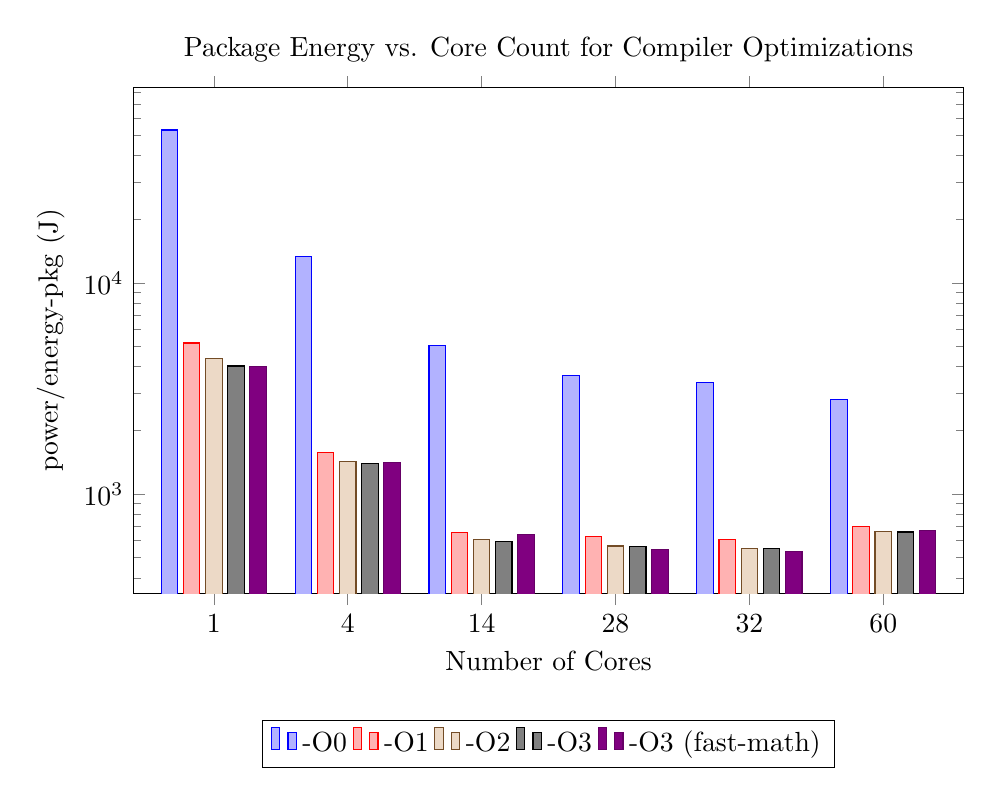
\begin{tikzpicture}
    \begin{axis}[
        title={Package Energy vs. Core Count for Compiler Optimizations},
        width=\textwidth,
        height=8cm,
        ybar,
        ymode=log,
        log basis y={10},
        enlarge x limits=0.12,
        xlabel={Number of Cores},
        ylabel={power/energy-pkg (J)},
        symbolic x coords={1, 4, 14, 28, 32, 60},
        xtick=data,
        bar width=6pt,
        legend style={
          at={(0.5,-0.25)},
          anchor=north,
          legend columns=-1
        },
        yticklabel style={
            /pgf/number format/fixed,
            /pgf/number format/precision=2
        },
    ]
    \addplot coordinates {(1, 52957.47) (4, 13379.59) (14, 5056.15) (28, 3650.43) (32, 3353.53) (60, 2794.03)};
    \addplot coordinates {(1, 5185.28) (4, 1564.51) (14, 658.46) (28, 627.89) (32, 606.52) (60, 698.96)};
    \addplot coordinates {(1, 4388.12) (4, 1417.01) (14, 606.58) (28, 565.83) (32, 552.98) (60, 661.76)};
    \addplot coordinates {(1, 4031.83) (4, 1386.60) (14, 595.29) (28, 561.59) (32, 548.83) (60, 659.31)};
    \addplot coordinates {(1, 4005.70) (4, 1414.08) (14, 639.00) (28, 547.56) (32, 535.22) (60, 671.51)};

    \legend{-O0, -O1, -O2, -O3, -O3 (fast-math)}
    \end{axis}
  \end{tikzpicture}
  \caption{Package consumption for multiple compiler flags}{Package energy consumption (log scale) for various core counts and compiler flags.}
  \label{fig:pkg-energy-chart}
\end{figure}

% --- Chart 3: RAM Energy ---
\begin{figure}[!ht]
  \centering
  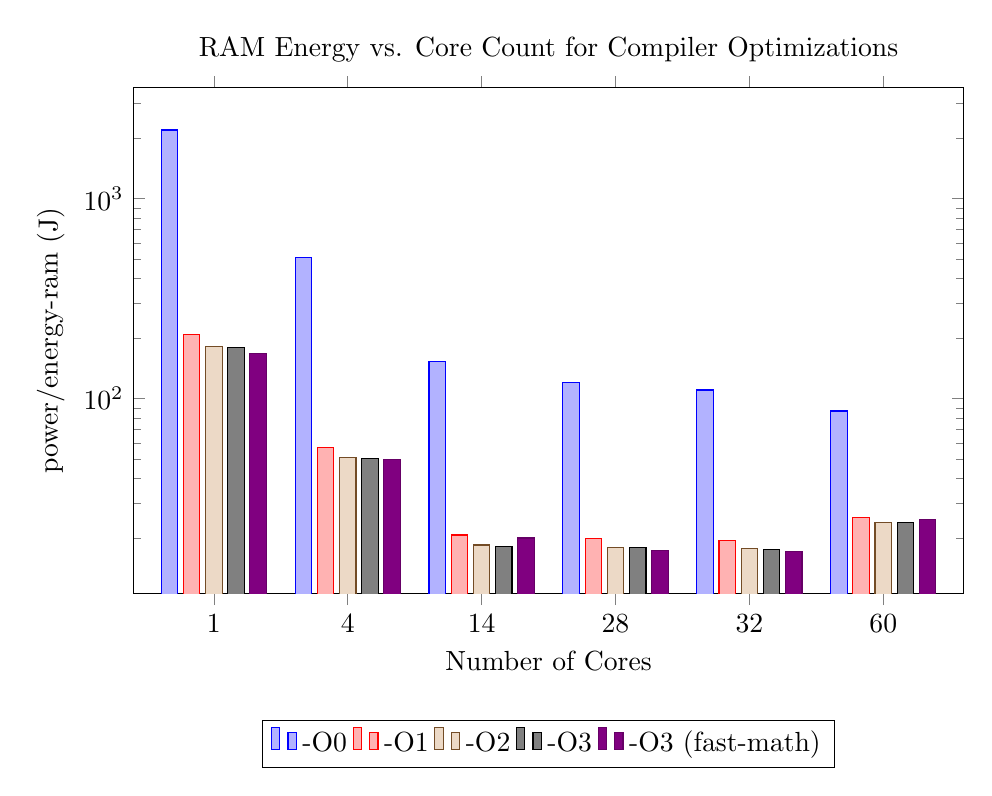
\begin{tikzpicture}
    \begin{axis}[
        title={RAM Energy vs. Core Count for Compiler Optimizations},
        width=\textwidth,
        height=8cm,
        ybar,
        ymode=log,
        log basis y={10},
        enlarge x limits=0.12,
        xlabel={Number of Cores},
        ylabel={power/energy-ram (J)},
        symbolic x coords={1, 4, 14, 28, 32, 60},
        xtick=data,
        bar width=6pt,
        legend style={
          at={(0.5,-0.25)},
          anchor=north,
          legend columns=-1
        },
        yticklabel style={
            /pgf/number format/fixed,
            /pgf/number format/precision=2
        },
    ]
    \addplot coordinates {(1, 2208.08) (4, 508.40) (14, 153.03) (28, 120.49) (32, 110.47) (60, 86.80)};
    \addplot coordinates {(1, 210.28) (4, 56.72) (14, 20.79) (28, 20.00) (32, 19.54) (60, 25.37)};
    \addplot coordinates {(1, 183.21) (4, 50.96) (14, 18.53) (28, 18.00) (32, 17.76) (60, 24.11)};
    \addplot coordinates {(1, 180.00) (4, 50.37) (14, 18.24) (28, 17.93) (32, 17.58) (60, 24.10)};
    \addplot coordinates {(1, 168.52) (4, 49.56) (14, 20.10) (28, 17.47) (32, 17.27) (60, 24.76)};

    \legend{-O0, -O1, -O2, -O3, -O3 (fast-math)}
    \end{axis}
  \end{tikzpicture}
  \caption{RAM consumption for multiple compiler flags}{RAM energy consumption (log scale) for various core counts and compiler flags.}
  \label{fig:ram-energy-chart}
\end{figure}


From the \autoref{tab:compiler-optimizations}, we can see that -O3 can be up to $13.13x$ more efficient and $11.44x$ faster than \texttt{-O0}, and \texttt{-O3} and $13.22x$ more efficient and $12.25x$ faster if we add the \texttt{--fast-math} flag on a single core task. But when we change and add more cores, the improvement decreases up to $4.24x$ faster more energy efficient and $4.16x$ faster with \texttt{-O3} and consume $4.22x$ less energy and take $4.11x$ less time with \texttt{-O3 --fast-math}.

Thus, we can see that the compiler optimizations play a very important role in the performance of the code, and that C++ is not always the most efficient language, as it depends on the compiler optimizations used. In conclusions, for optimization flags, even though \texttt{-O3 with --fast-math} is the most efficient, I would recommend using \texttt{-O3} for high-performance computing, as it provides a good balance between performance and accuracy. If the program is just a regular program, I would recommend using \texttt{-O2}, as it provides a good balance between performance and code size as well as compilation time, which we have not taken into account as the program is just compiled once and may be executed thousands of times.